\documentclass[11pt,a4paper]{article}
\usepackage{fontspec}
\setmainfont{Source Serif 4}[Path=/home/claude/ref/fonts/, UprightFont=SourceSerif4-Regular.ttf, BoldFont=SourceSerif4-Semibold.ttf, ItalicFont=SourceSerif4-It.ttf]
\setmonofont{IBM Plex Mono}[Path=/home/claude/ref/fonts/, UprightFont=IBMPlexMono-Regular.ttf, BoldFont=IBMPlexMono-Medium.ttf, Scale=0.88]
\usepackage[a4paper,margin=2.4cm]{geometry}
\usepackage{amsmath}
\usepackage{graphicx,booktabs,float,caption,array,xcolor,longtable}
\usepackage{xurl}
\usepackage[hidelinks]{hyperref}
\usepackage[round]{natbib}
\usepackage{setspace}
\setstretch{1.08}
\renewcommand{\topfraction}{0.9}
\renewcommand{\bottomfraction}{0.8}
\renewcommand{\textfraction}{0.1}
\renewcommand{\floatpagefraction}{0.75}
\setlength{\parindent}{0pt}
\setlength{\parskip}{0.55em}
\captionsetup{font=small,labelfont=bf}
\setlength{\bibsep}{3pt}
\urlstyle{same}
\hypersetup{pdftitle={Do By-Elections Make Parliament Listen?},pdfauthor={Dr Tristan Hotham}}

\begin{document}
\begin{center}
{\Large\bfseries Do By-Elections Make Parliament Listen? Parliamentary Attention to By-Election Constituencies in the House of Commons, 1911 to 2023\par}
\vspace{1.2em}
{\large Dr Tristan Hotham\par}
\vspace{0.3em}
{\small Independent researcher\\
ORCID: 0000-0003-4931-9349\\
DOI: https://doi.org/10.5281/zenodo.24094210\par}
\vspace{0.8em}
2026
\end{center}

\begin{quote}
\small
\begin{center}\textbf{Abstract}\end{center}
By-elections are among the most visible events in British politics, yet we know little about whether they change what Parliament talks about. I link every UK by-election from 1909 in the Wikipedia lists (1,339) to monthly counts of House of Commons contributions that say ``in'' a town named in the seat, from the Hansard API. In a stacked event study fixed in a written analysis plan before any outcome was examined, each of 387 by-election towns (366 by-elections, 1912 to 2022) is compared with five matched towns in the same months, using Poisson pseudo-maximum likelihood with errors clustered by by-election. Mentions rise in the three months before polling (by 81\%, 95\% CI 26 to 159), peak in the polling month and the two after (296\%, CI 196 to 429), and remain higher three to twelve months later (91\%, CI 51 to 143) and in the second year (55\%, CI 19 to 101); the third-year difference is not distinguishable from zero. Placebo dates, neighbouring towns and the seat-name phrase show no comparable rise. The initial jump is larger when the seat changes hands, but the later attention is not. No rise is detectable before 1945, and the rise is largest after 1980. The design is observational: it measures the attention that comes with the whole episode of vacancy, campaign and new member, not the effect of the vote alone.

\textbf{Keywords:} by-elections; parliamentary attention; constituency representation; House of Commons; Hansard; event study
\end{quote}

\section{Introduction}
British by-elections are small events with large audiences. A vacancy in one of 600-odd seats can dominate a month of political news, and a lost by-election can unsettle a government for far longer. A large literature asks what by-elections reveal about national opinion: whether governments lose them because of mid-term disillusion, turnout, or tactical protest \citep{mughan1986,mughan1988,price1998}, whether they work as referenda on the government \citep{feigert1990}, how they compare with special elections elsewhere \citep{studlar1987,loewen2010}, whether they forecast or shape the next general election \citep{upton1991,hanretty2021}, and how they have changed over the century \citep{pollock1941,norris1990,cook1997}. All of this treats the by-election as a signal sent from voters to the parties. Much less is known about what happens in the other direction: whether, once the result is in, the place that held the by-election receives more attention from Parliament.

That question matters for theories of representation. If members of the House of Commons are responsive to electoral threat \citep{andre2015,kellermann2016} and if constituency service has become a larger part of the job \citep{cain1987,norton1993,norton1994}, then a by-election, which concentrates national attention and electoral uncertainty on one constituency, should raise the salience of that constituency in the chamber. A new member arrives with a mandate to speak for the place, parties that won or lost there have reasons to keep referring to it, and ministers may be asked about local problems the campaign exposed. On the other hand, the House's agenda is crowded and set mostly by government business, and the extra attention of a campaign could vanish with the television crews.

This paper measures the parliamentary attention that follows a by-election. I parse the Wikipedia lists of United Kingdom by-elections from 1900 to the present, link each seat to the towns in its name, and count, month by month from 1909 to 2026, how many House of Commons contributions say ``in'' each town, using the Hansard API. The design is a stacked event study \citep{cengiz2019}: each by-election town is followed from two years before to three years after polling day and compared with five towns of similar size and prior attention that had no by-election, in the same calendar months. The specification, the reference period, the exclusions and the checks were written down in an analysis plan before any outcome model was run (Section~\ref{sec:design}).

The main findings are clear. Commons mentions of a by-election town rise in the three months before polling, when the seat is vacant and the campaign is under way, peak in the polling month and the two after at about 4.0 times the level of matched towns, and remain about 1.9 times higher three to twelve months later and 1.6 times higher in the second year. By the third year the difference (1.31 times) is no longer distinguishable from zero and is significant in only 7 of 18 robustness checks. Placebo dates two years earlier, neighbouring towns outside the seat, and the seat's own name (which rises mechanically when a new member is called ``the hon. Member for'' the seat) show nothing comparable. A seat changing hands roughly doubles the immediate jump, but not the lasting attention. And the whole pattern is a post-war phenomenon: there is no detectable rise for by-elections between 1911 and 1944.

The contribution is threefold. First, it moves the study of by-elections from what they say about voters to what they do to Parliament's agenda, connecting a long British literature to work on representation and attention \citep{eulau1977,jones2005}. Second, it offers a new, transparent measure of geographic attention in the Commons over more than a century, built from counts that anyone can re-run, and a design that compares each place with itself and with matched places month by month. Third, it shows that this kind of responsiveness has a history: the link between a constituency's electoral moment and its place in debate appears to have been forged after 1945, consistent with accounts of the growth of the constituency role of MPs \citep{norton1994,norton1993}.

The rest of the paper is organised as follows. Section~\ref{sec:lit} reviews work on by-elections and on constituency representation in parliamentary speech. Section~\ref{sec:data} describes the data. Section~\ref{sec:design} sets out the pre-specified design. Section~\ref{sec:results} reports the results and Section~\ref{sec:robust} the placebo and robustness checks. Section~\ref{sec:disc} discusses mechanisms and limitations, and Section~\ref{sec:conc} concludes.

\section{Background and literature}\label{sec:lit}
\subsection{By-elections in British politics}
By-elections fill vacancies between general elections. In the United Kingdom they are triggered by a member's death, resignation (formally, appointment to an office of profit under the Crown), elevation to the peerage, disqualification, expulsion, a successful recall petition, or, until 1926, appointment to ministerial office, which obliged a member to seek re-election. Their political weight has long been recognised. \citet{pollock1941} surveyed the by-elections between the wars, and the edited collection of \citet{cook1997} traces their role and influence in British politics since 1918. In his introduction to its first edition, as \citet{upton1991} recalls, David Butler suggested that by-elections ``may offer some guide to the public mood'' while doubting that anyone could estimate how far a result departs from what a general election held the same day would produce.

Most quantitative work since has asked what by-elections reveal about voters. \citet{mughan1986} noted the ``almost invariable loss of support experienced by governments relative to the preceding general election'' and tested turnout, referendum and personal-vote explanations, finding that their combination matters; \citet{mughan1988} returned to the government's by-election vote. \citet{price1998} argued that if voters care about the size of the government's majority and weigh the downside of their least-preferred party winning more heavily, governments will tend to lose by-elections even without a change in national support, and tested this against post-war contests. \citet{feigert1990} asked, across four countries, whether by-elections constitute referenda on the government, and \citet{studlar1987} compared British by-elections with American special elections, which had attracted far less attention. \citet{norris1990} offered a book-length account of the volatile by-election electorate. Later work asked whether by-election results carry over to general elections \citep{upton1991} and whether they can be forecast: \citet{hanretty2021} trains a Dirichlet regression on all 468 post-war UK by-elections and achieves accuracy close to that of by-election polls. Outside Britain, \citet{loewen2010} ask whether Canadian federal by-elections between 1963 and 2008 are significant at all.

This literature is about electoral behaviour. Its implicit model is of by-elections as messages from voters to parties and governments. What those messages do once they arrive has received much less systematic study, beyond case histories of famous upsets. If governments read by-elections as signals, one place where the signal could show is in the parliamentary agenda: in how often the place, its problems and its new member appear in debate.

\subsection{Constituency representation and attention in Parliament}
A second literature concerns the territorial side of representation. \citet{eulau1977} distinguished policy, service, allocation and symbolic responsiveness, and \citet{mansbridge2003} widened the notion of representation to include anticipatory, gyroscopic and surrogate forms, with standards that are systemic rather than dyadic. In the United States, \citet{fenno1978} showed how members' perceptions of their constituencies shape their behaviour at home and in Washington. \citet{cain1987} compared the personal vote and constituency service in the United States and Britain, arguing that British members were moving towards an ombudsman role. \citet{norton1993} documented the growth of British MPs' constituency work and its electoral importance, and \citet{norton1994} described ``the growth of the constituency role of the MP''. \citet{searing1985,searing1994} studied the role of the good constituency member among the roles MPs adopt at Westminster.

Recent work measures constituency focus in what legislators say and ask. Parliamentary questions have been the main instrument: \citet{martin2011} uses them to measure constituency focus in Ireland, \citet{russo2011} in Italy, \citet{zittel2019} in the German Bundestag using quantitative text analysis, and \citet{kellermann2016} relates electoral vulnerability to constituency focus in House of Commons questions. \citet{soroka2009} find that Canadian MPs' contributions to Question Period reflect the preferences of their geographic constituencies. \citet{andre2015} show in fourteen countries that electoral vulnerability mediates the effect of electoral institutions on legislators' constituency effort, and \citet{fernandes2018} find that representation focus in Portuguese parliamentary questions changes with the electoral cycle and with vulnerability. At the level of governments, \citet{hobolt2008} find that greater political contestation goes with more responsive executive speeches and spending in Britain, Denmark and the United States. Attention itself is scarce: \citet{jones2005} model how governments allocate it across problems. And debate records are now routinely analysed at scale; \citet{rheault2016}, for example, track emotional tone across a century of UK parliamentary debates.

\subsection{What is new here}
These literatures rarely meet. Studies of by-elections focus on vote shares; studies of constituency focus usually compare members or seats cross-sectionally, or follow members through the electoral cycle. The by-election is an attractive design for the second question because it is a sharp, dated, local event, and because the British record allows it to be observed in hundreds of places over a century. This paper is, as far as I can find, the first to measure systematically whether parliamentary attention to a place changes when its seat holds a by-election, how long any change lasts, and how it varies with the kind of by-election and the era. It uses an outcome, mentions of the town ``in'' Commons speech, that does not depend on who asks or answers, and a design that compares each place with matched places in the same calendar months.

\section{Data}\label{sec:data}
\subsection{By-elections}
The list of by-elections comes from the six English Wikipedia pages ``List of United Kingdom by-elections'' covering 1900 to 1918, 1918 to 1931, 1931 to 1950, 1950 to 1979, 1979 to 2010 and 2010 to the present \citep{wikipedia2026}, retrieved in 2026. I parsed the wikitext of every table row (1,530 by-elections from 1900; 1,339 from 1909, the first year of the Hansard series used here): seat, date, incumbent and party, winner and party, and the stated cause. Rows that the lists shade are those where the seat changed party; this agrees with a comparison of the two parties' families in 98.9\% of cases. Party labels were mapped to families, keeping Coalition Liberals apart for 1918 to 1922 and counting Ulster Unionists with the Conservatives until 1972. The governing parties at each date, including coalitions and the National Government, were coded by hand, which gives whether the seat was government-held and whether the government lost it.

Causes were grouped from the cause text: death; resignation and appointments (including peerages, judicial and other offices, and ill health); scandal or a voided election (expulsion, conviction, bankruptcy, disqualification, recall, an election declared void, or resignation in a scandal; every case was read by eye); and re-election of the same member, which covers ministerial re-elections before 1926 and later recontests such as the Ulster Unionist resignations of 1986. Uncontested by-elections are those noted as such in the lists. As a check on coverage, 935 of the 1,339 by-elections since 1909 (69.8\%) have a Wikidata item of type by-election with the same seat name and year, with the same date in 98.3\% of those; the 16 Wikidata items not matched are all spelling variants of seats that are in the lists (for example ``Hull North'' for Kingston upon Hull North). Figure~\ref{fig:timeline} shows the by-elections per year.

\begin{figure}[tbp]\centering
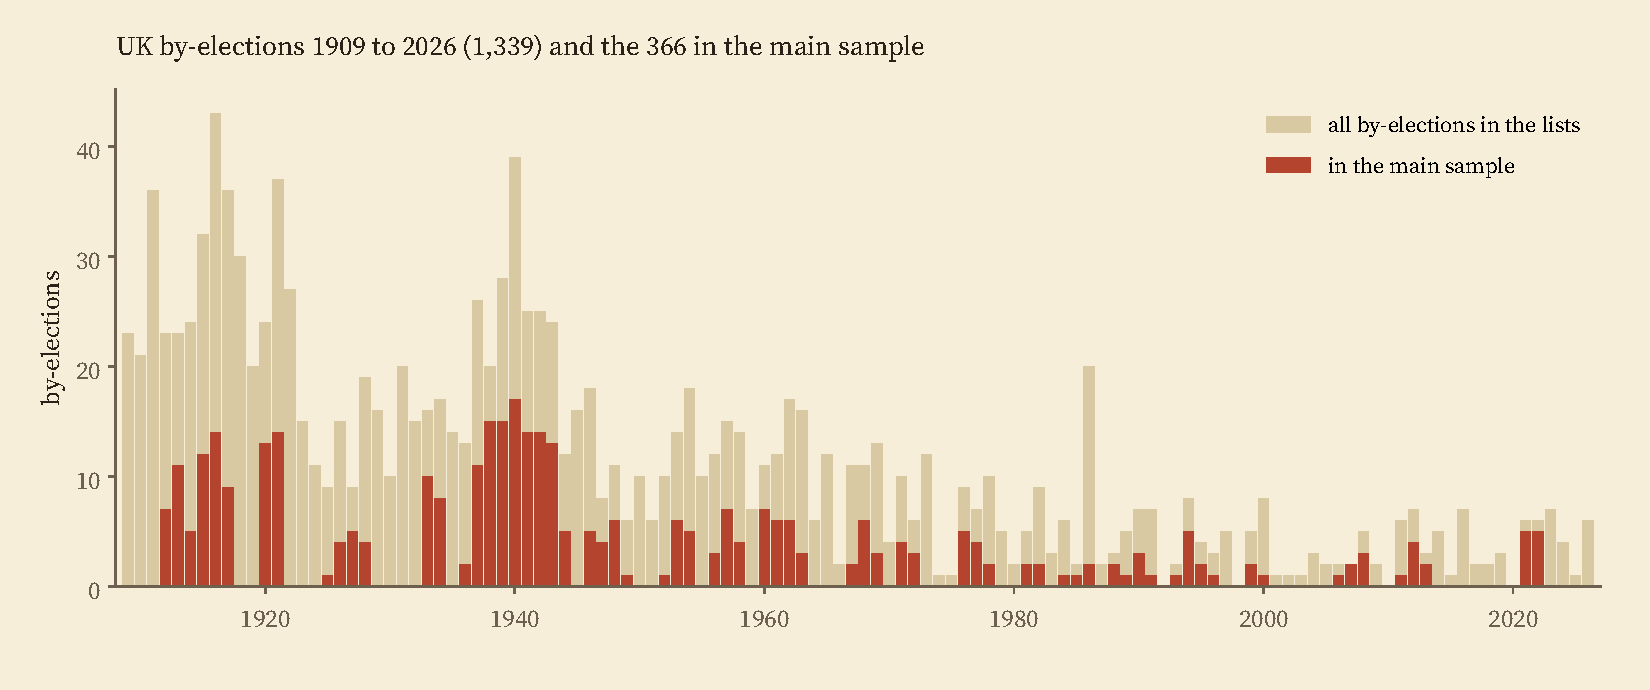
\includegraphics[width=\textwidth]{f_timeline.pdf}
\caption{UK by-elections per year in the Wikipedia lists, 1909 to 2026, and those in the main sample. The main sample excludes by-elections within twelve months of a general election, those too early or too late for the five-year window, and others (Table~\ref{tab:flow}).}\label{fig:timeline}
\end{figure}

\subsection{Parliamentary attention}
The outcome is the number of House of Commons contributions in a month whose text contains the phrase ``in'' plus a town's name, from the timeline statistics of the UK Parliament Hansard API (contribution type Spoken, grouped by month, 1909 to October 2026). The counts are of contributions, not of words. The 1,661 town names, their points, populations and ambiguity flags come from my earlier study \textit{Mentioned in the House} \citep{hotham2026a}, which used the same phrase: it avoids the formula ``the hon. Member for'', surnames, and division lists, and it is a sample of all the ways a place can be mentioned. Names that are shared by two UK places, used for a better-known namesake (Boston, Perth, Durham) or ordinary words are flagged there and are not used here. Longer names that begin with a shorter one (``in Bury St Edmunds'' is also counted as ``in Bury'') are subtracted month by month, and spelling variants are added to their main form. The last complete month is September 2026.

The same API also gives monthly counts of contributions containing each by-election seat's own name. This phrase is used as a secondary outcome only, because it is mechanically raised when a new member is referred to as ``the hon. Member for'' the seat (Section~\ref{sec:robust}).

\subsection{Linking seats to towns}
Each seat name was searched for town names as whole words, taking the longest non-overlapping matches: ``Batley and Morley'' gives Batley and Morley; ``Bury St Edmunds'' gives Bury St Edmunds, not Bury; ``The Hartlepools'' gives Hartlepool. University seats were dropped. Every link was checked against the seat's point from \textit{Who Won Here?} \citep{hotham2026b}: links more than 60 km away were dropped as different places, and all links over 12 km were read by eye. Four further links were removed by hand (Colne Valley is not Colne; Liverpool West Derby is not Derby; Plymouth Sutton is not Sutton in London; Kincardine and Deeside is not Deeside in Flintshire) and three kept with corrected points. In all, 957 by-elections since 1909 are linked to at least one town (1,006 links). The others are mostly county divisions named after a county or district rather than a town (``Mid Bedfordshire'', ``South Molton'' and the like) or Irish seats before 1922.

The town in a seat's name is not the same as the seat. A borough seat such as Kettering covers the town and its surroundings; a division such as Bradford South covers part of a larger town. Seats in cities with many divisions are a small part of the place whose name is counted, so their by-elections should move the count much less. I therefore record, for each link, how many seats at the preceding general election contain the town's name, and the main sample keeps towns named in at most two seats (Section~\ref{sec:design}).

\begin{table}[tbp]\centering\small\caption{From by-elections to the main sample.}\label{tab:flow}\begin{tabular}{lr}\toprule Step & Number\\\midrule
By-elections in the Wikipedia lists, 1909 to 2026 & 1,339\\
\quad university seats & 25\\
\quad linked to at least one Hansard town & 957\\
By-election towns (links) & 1,006\\
\quad less: town name ambiguous in Hansard & $-$63\\
\quad less: window outside the data (polling before 1911 or after September 2023) & $-$38\\
\quad less: same member re-elected (used as a placebo) & $-$51\\
\quad less: within 12 months of a general election & $-$332\\
\quad less: another by-election naming the town within the window & $-$77\\
\quad less: town named in three or more seats & $-$58\\\midrule
Main sample: by-election towns & 387\\
\quad by-elections & 366\\
\quad distinct towns & 253\\
\quad distinct control towns & 701\\
\quad town-months in the stacked panel & 141,642\\\bottomrule\end{tabular}\end{table}

\subsection{Matched comparison towns}
For each by-election town, I selected five comparison towns from the same nation (from all nations if fewer than fifteen were eligible) that were not named in any seat holding a by-election within the window and twelve months either side, were more than 25 km from every town of that by-election, and were nearest on two variables: the log of one plus the mean monthly mentions in the reference months (24 to 13 months before polling) and log population, weighted two to one. Matching used only the reference months, which are also the baseline of the comparison; no information from the months around or after polling was used. Controls are chosen without replacement within a by-election and may serve different by-elections. In the main sample 701 different towns serve as controls.

\section{Research design}\label{sec:design}
\subsection{Analysis plan}
The analysis plan was written in the project notes before any outcome model was run, after the data construction described above. It fixed the unit (a by-election town and its controls), the outcome, the window (24 months before to 36 after polling), the reference period (months $-24$ to $-13$, before any plausible vacancy), the bins, the estimator and clustering, six hypotheses, and every check reported in Section~\ref{sec:robust}. The plan was not registered with a third party, and I report it as pre-specified in a written plan. Analyses added later are labelled exploratory.

The hypotheses were: (H1) mentions of a by-election town rise around the by-election; (H2) the rise outlasts the campaign, into the first, second and third years; (H3) the rise is larger when the seat changes hands, and when the government loses it; (H4) it differs by cause; (H5) it differs by era (1911 to 1944, 1945 to 1979, 1980 to 2023); and (H6) it differs between government-held and opposition-held seats. H1 would be contradicted by a confidence interval for the polling period that includes zero; H2 by intervals including zero for the later bins. H3 to H6 were tested two-sided.

\subsection{Sample}
The main sample applies, in this order: towns flagged as ambiguous are dropped; the full window must lie within the data (polling between January 1911 and September 2023); re-elections of the same member are set aside (they are used as a placebo); by-elections within twelve months of a general election are excluded, because the general election would move attention everywhere and change the member; a town with another by-election in a seat naming it within the window is excluded; and towns named in more than two seats at the preceding general election are excluded. Table~\ref{tab:flow} shows the flow. The main sample has 387 by-election towns from 366 by-elections (21 by-elections name two towns) in 253 distinct towns. Table~\ref{tab:desc} describes it.

\begin{table}[tbp]\centering\small\caption{The main sample by era. Mentions are mean ``in'' contributions per town in the reference year (months $-24$ to $-13$) and in the polling month and the twelve after (months 0 to 12), for by-election towns and their controls (per control town).}\label{tab:desc}\setlength{\tabcolsep}{4pt}\begin{tabular}{lrrrrrrrr}\toprule & & & Changed & & \multicolumn{2}{c}{By-election towns} & \multicolumn{2}{c}{Controls}\\\cmidrule(lr){6-7}\cmidrule(lr){8-9}Era & Towns & By-elections & hands (\%) & Death (\%) & Ref. & After & Ref. & After\\\midrule
1911 to 1944 & 230 & 223 & 17 & 47 & 0.76 & 1.13 & 0.38 & 0.37\\
1945 to 1979 & 99 & 93 & 13 & 42 & 1.63 & 4.12 & 1.52 & 1.72\\
1980 to 2023 & 58 & 50 & 41 & 64 & 4.14 & 13.69 & 3.90 & 3.63\\
\midrule
All & 387 & 366 & 20 & 48 & 1.49 & 3.78 & 1.20 & 1.21\\
\bottomrule\end{tabular}\end{table}

\subsection{Main specification}
Let $y_{ust}$ be the count of ``in'' mentions of town $u$ in stack $s$ (one stack per by-election, containing its by-election towns and their controls) in calendar month $t$, and $k = t - t_s$ the month relative to polling. The main model (M1) is a Poisson pseudo-maximum likelihood regression
\begin{equation}
E[y_{ust}] = \exp\Big(\alpha_{us} + \gamma_{st} + \sum_{b} \beta_b \, D_{us} \, \mathbf{1}[k \in b]\Big),
\end{equation}
where $\alpha_{us}$ are town-within-stack fixed effects, $\gamma_{st}$ are stack-by-calendar-month fixed effects, $D_{us}$ marks the by-election town, and the bins $b$ are months $-12$ to $-4$ (pre), $-3$ to $-1$ (vacancy and campaign), $0$ to $2$ (result), $3$ to $12$ (year 1), $13$ to $24$ (year 2) and $25$ to $36$ (year 3), with months $-24$ to $-13$ as the reference. Because $\gamma_{st}$ is specific to each stack and month, every by-election town is compared only with its own controls in the same month; the stacked structure avoids the problems of two-way fixed-effects estimators with staggered timing \citep{baker2022,sun2021,cengiz2019}. PPML handles the many zero counts and is consistent under heteroskedasticity where a log-linear model is not \citep{santos2006}; it is estimated with the iteratively reweighted least squares algorithm with high-dimensional fixed effects described by \citet{correia2020}, as implemented in the Python package pyfixest. Units with no mentions in the whole window, and stack-months in which no town is mentioned, carry no information and drop out. Standard errors are clustered by by-election \citep{cameron2015,abadie2023}. Coefficients are reported as percentage changes, $100(\exp(\beta_b)-1)$, with 95\% confidence intervals. A monthly version replaces the bins with one indicator for each month from $-12$ to $36$.

Heterogeneity is estimated by interacting the bins (with months 13 to 36 pooled as ``later'') with group indicators in the same stacked model, which gives an estimate for each group and contrasts with their own standard errors.

\subsection{Threats to inference}
By-elections are not random events. Deaths may follow long illness, during which a member speaks less; resignations may follow scandal or appointment; both may themselves be news that raises mentions before the by-election. The design compares a town with itself before the vacancy and with similar towns in the same months, so it removes stable differences between places and common shocks to Parliament's attention, but not events specific to the place that cause both the vacancy and the attention. The estimand is therefore the change in attention that accompanies the whole episode, from vacancy through campaign and result to the new member's first years, not the causal effect of the vote. The pre-period bin ($-12$ to $-4$) tests for drift before the vacancy, the placebo with dates moved two years earlier tests whether the method finds effects where there should be none, and the neighbouring-towns placebo tests for regional news shocks.

Measurement is a second concern. The phrase ``in'' plus a town's name can also refer to the constituency (``the by-election in Kettering''). That is parliamentary attention to the place in the sense intended here, but it means the measure cannot separate talk about the town from talk about the contest. The seat-name phrase, used as a secondary outcome, shows how much of the change is the formal naming of the member.

\section{Results}\label{sec:results}
\subsection{Main estimates}
Figure~\ref{fig:event}A shows the raw pattern. Each series is the mean monthly count divided by its own mean in the reference months. Matched towns are flat; by-election towns are flat until three months before polling, then rise sharply to about 6.6 times their reference level in the polling month, and stay above it. In absolute terms, by-election towns were mentioned 0.12 times a month on average in the reference months (about 1.5 times a year), 0.82 times in the polling month, and 0.22 times a month in months 3 to 12, against 0.09 for their controls.

\begin{figure}[tbp]\centering
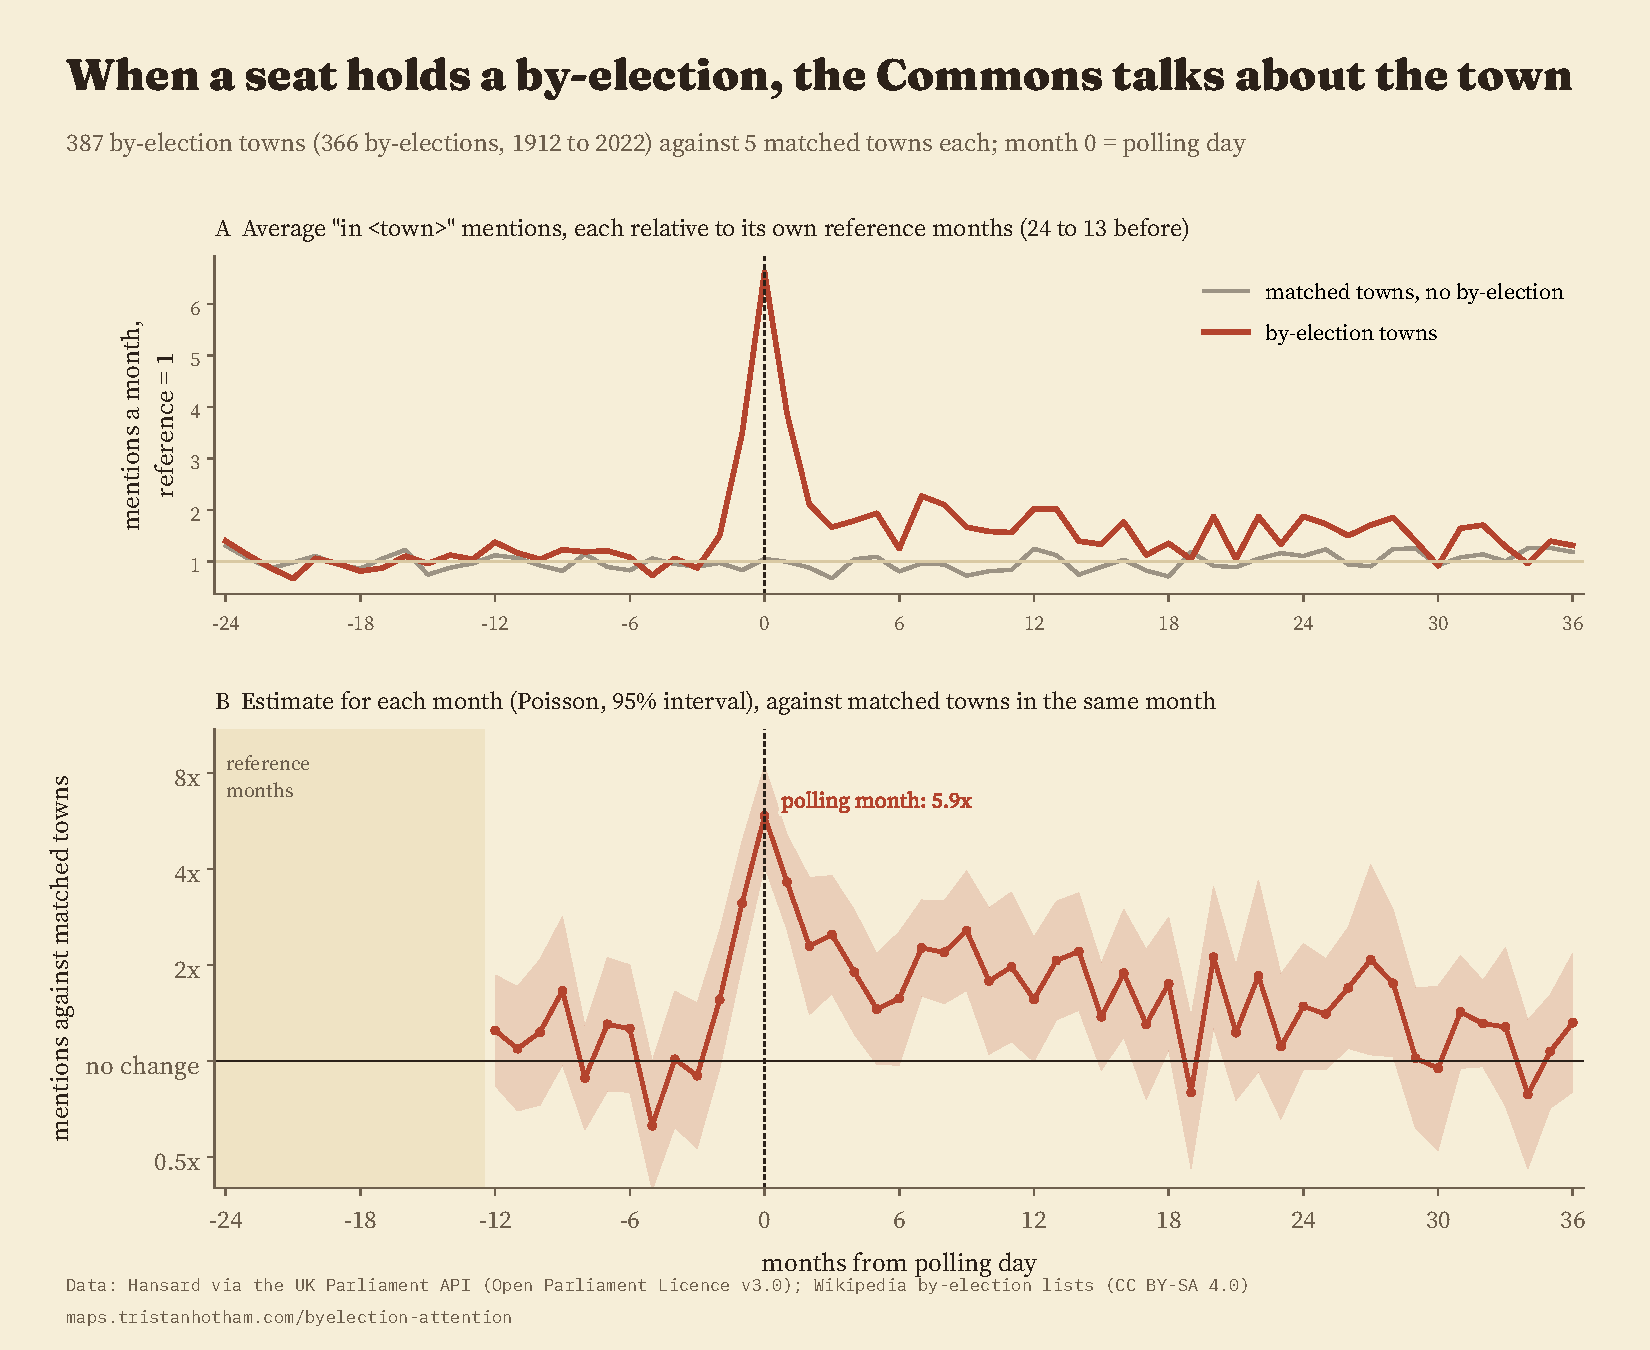
\includegraphics[width=\textwidth]{f_event.pdf}
\caption{Commons ``in'' mentions of by-election towns and matched towns, months $-24$ to $+36$ around polling. A: mean monthly count, each series relative to its own mean in the reference months. B: monthly PPML estimates from the event-study version of M1 with 95\% confidence intervals (errors clustered by by-election). $N$ = 387 by-election towns.}\label{fig:event}
\end{figure}

Table~\ref{tab:main} reports M1. There is no detectable drift before the vacancy: the pre bin is 12\% (95\% CI $-$11 to 40). In the three months before polling, mentions are 81\% higher than in matched towns (CI 26 to 159). In the polling month and the two after they are 296\% higher (CI 196 to 429), that is 3.96 times. H1 is supported. The rise lasts: three to twelve months after polling, mentions are 91\% higher (CI 51 to 143), and in the second year 55\% higher (CI 19 to 101). In the third year the estimate is 31\% with a confidence interval from $-$1 to 73. H2 is therefore supported for the first two years and not for the third. Pooling the six months around polling ($-3$ to $+2$) gives 192\% (CI 124 to 282), and pooling months 13 to 36 gives 42\% (CI 10 to 83).

\begin{table}[tbp]\centering\small\caption{Main model (M1): PPML of monthly ``in'' mentions with town-within-stack and stack-by-month fixed effects; reference months $-24$ to $-13$; standard errors clustered by by-election. Percentages are $100(\exp(b)-1)$ with 95\% confidence intervals.}\label{tab:main}\begin{tabular}{lrrlr}\toprule Period & $b$ & (SE) & \% [95\% CI] & $p$\\\midrule
Months $-12$ to $-4$ & 0.110 & (0.115) & 12 [$-$11, 40] & 0.335\\
Months $-3$ to $-1$ (vacancy) & 0.593 & (0.182) & 81 [26, 159] & 0.001\\
Months 0 to 2 (result) & 1.376 & (0.148) & 296 [196, 429] & 0.000\\
Months 3 to 12 & 0.648 & (0.121) & 91 [51, 143] & 0.000\\
Months 13 to 24 & 0.437 & (0.134) & 55 [19, 101] & 0.001\\
Months 25 to 36 & 0.270 & (0.143) & 31 [$-$1, 73] & 0.060\\
\midrule Pooled $-3$ to $+2$ (M1b) & 1.072 & (0.136) & 192 [124, 282] & 0.000\\
Pooled 13 to 36 (M1b) & 0.349 & (0.130) & 42 [10, 83] & 0.007\\
\midrule By-election towns & \multicolumn{4}{l}{387 (296 with any mention in the window)}\\
By-elections (clusters) & \multicolumn{4}{l}{366}\\
Town-months used / in panel & \multicolumn{4}{l}{28,621 / 141,642}\\\bottomrule\end{tabular}\end{table}

The monthly estimates in Figure~\ref{fig:event}B (listed in Appendix Table~\ref{tab:es}) show the shape: the estimate for the polling month itself is 487\% (CI 308 to 744), for the month before 213\%, and for the month after 264\%. Thereafter the monthly estimates settle around twice the matched level for about two years, with 8 of the 24 monthly estimates from months 13 to 36 individually above zero. Before the vacancy, 1 of the 9 monthly estimates from months $-12$ to $-4$ is individually different from zero at the 5\% level, as expected by chance.

Figure~\ref{fig:cases} illustrates individual by-elections. Orpington, after the Liberal gain there in 1962, was mentioned 0 times in the reference year and 13 times in the polling month and twelve after; Crewe, after the Conservative gain of Crewe and Nantwich in 2008, went from 2 to 50; Corby in 2012 from 4 to 54. Single by-elections are noisy, with few mentions on either side, which is why the analysis pools them; Figure~\ref{fig:map} maps the per-town ratio of mentions in the year after to the reference year, relative to the same ratio for the town's controls, and shows both rises and falls everywhere.

\begin{figure}[tbp]\centering
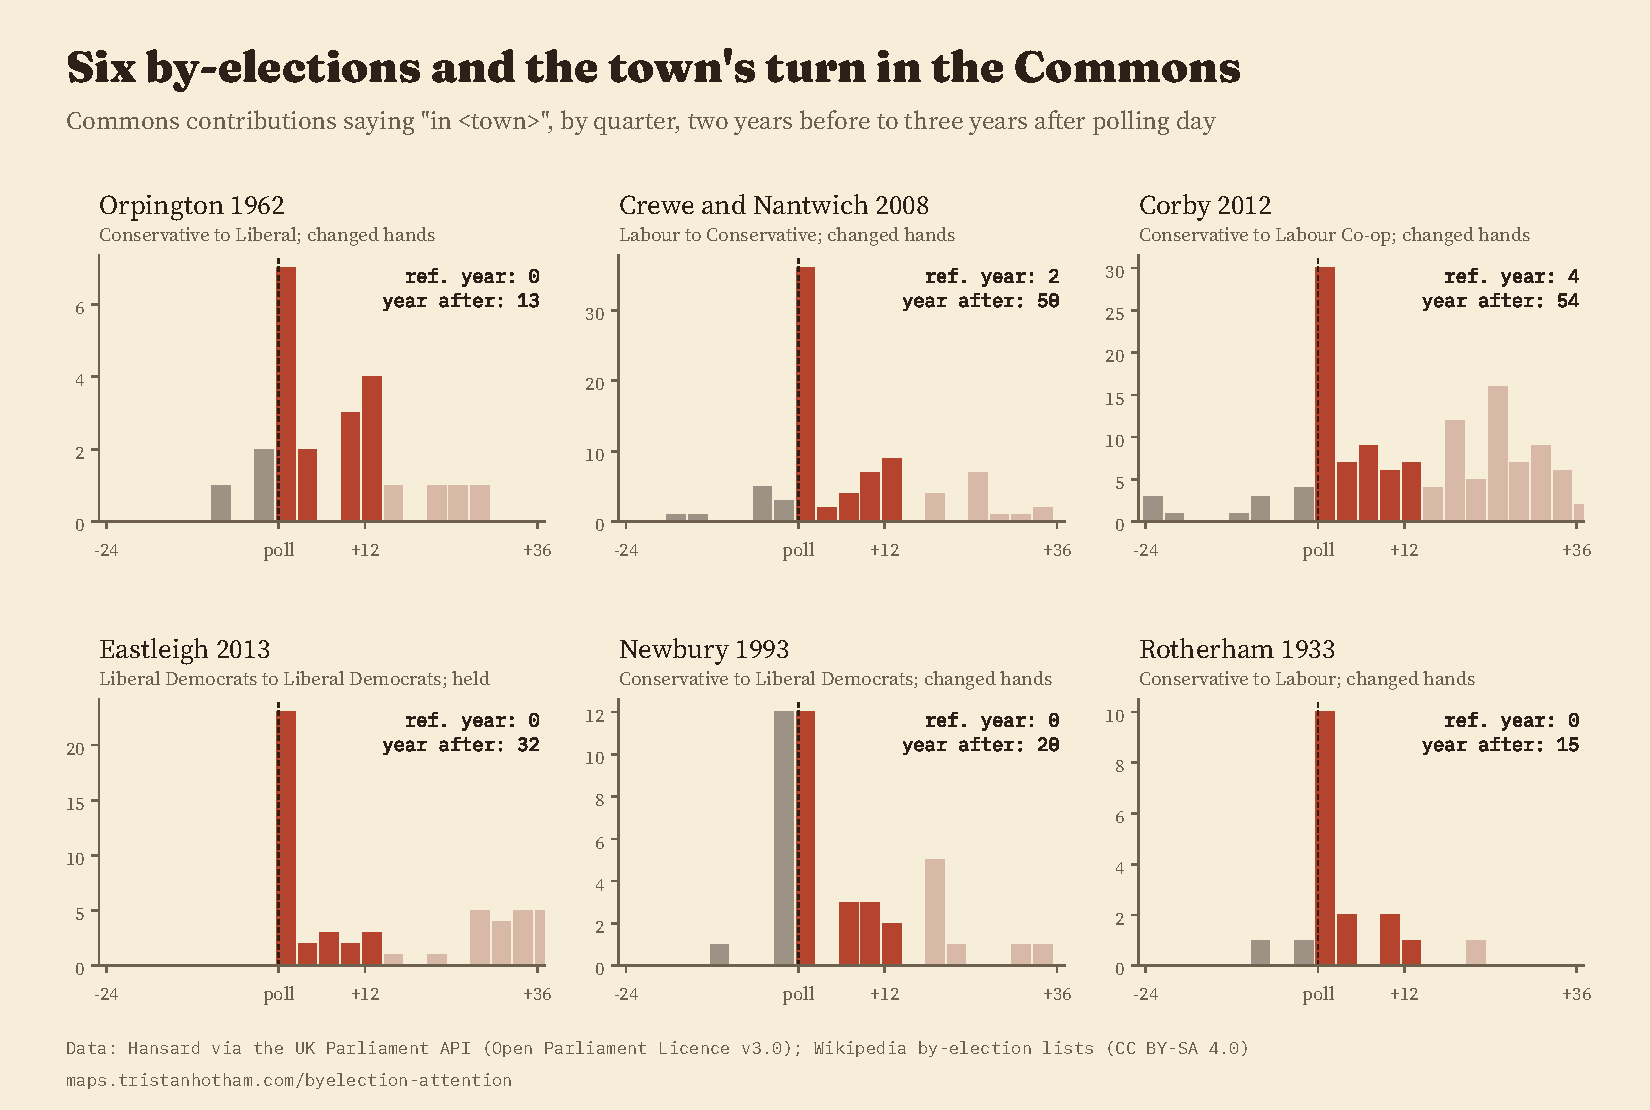
\includegraphics[width=\textwidth]{f_cases.pdf}
\caption{Quarterly ``in'' mentions of six by-election towns, from two years before to three years after polling. Grey: before polling; red: polling month to month 12; pale red: months 13 to 36. ``Ref. year'' is months $-24$ to $-13$; ``year after'' is months 0 to 12.}\label{fig:cases}
\end{figure}

\begin{figure}[tbp]\centering
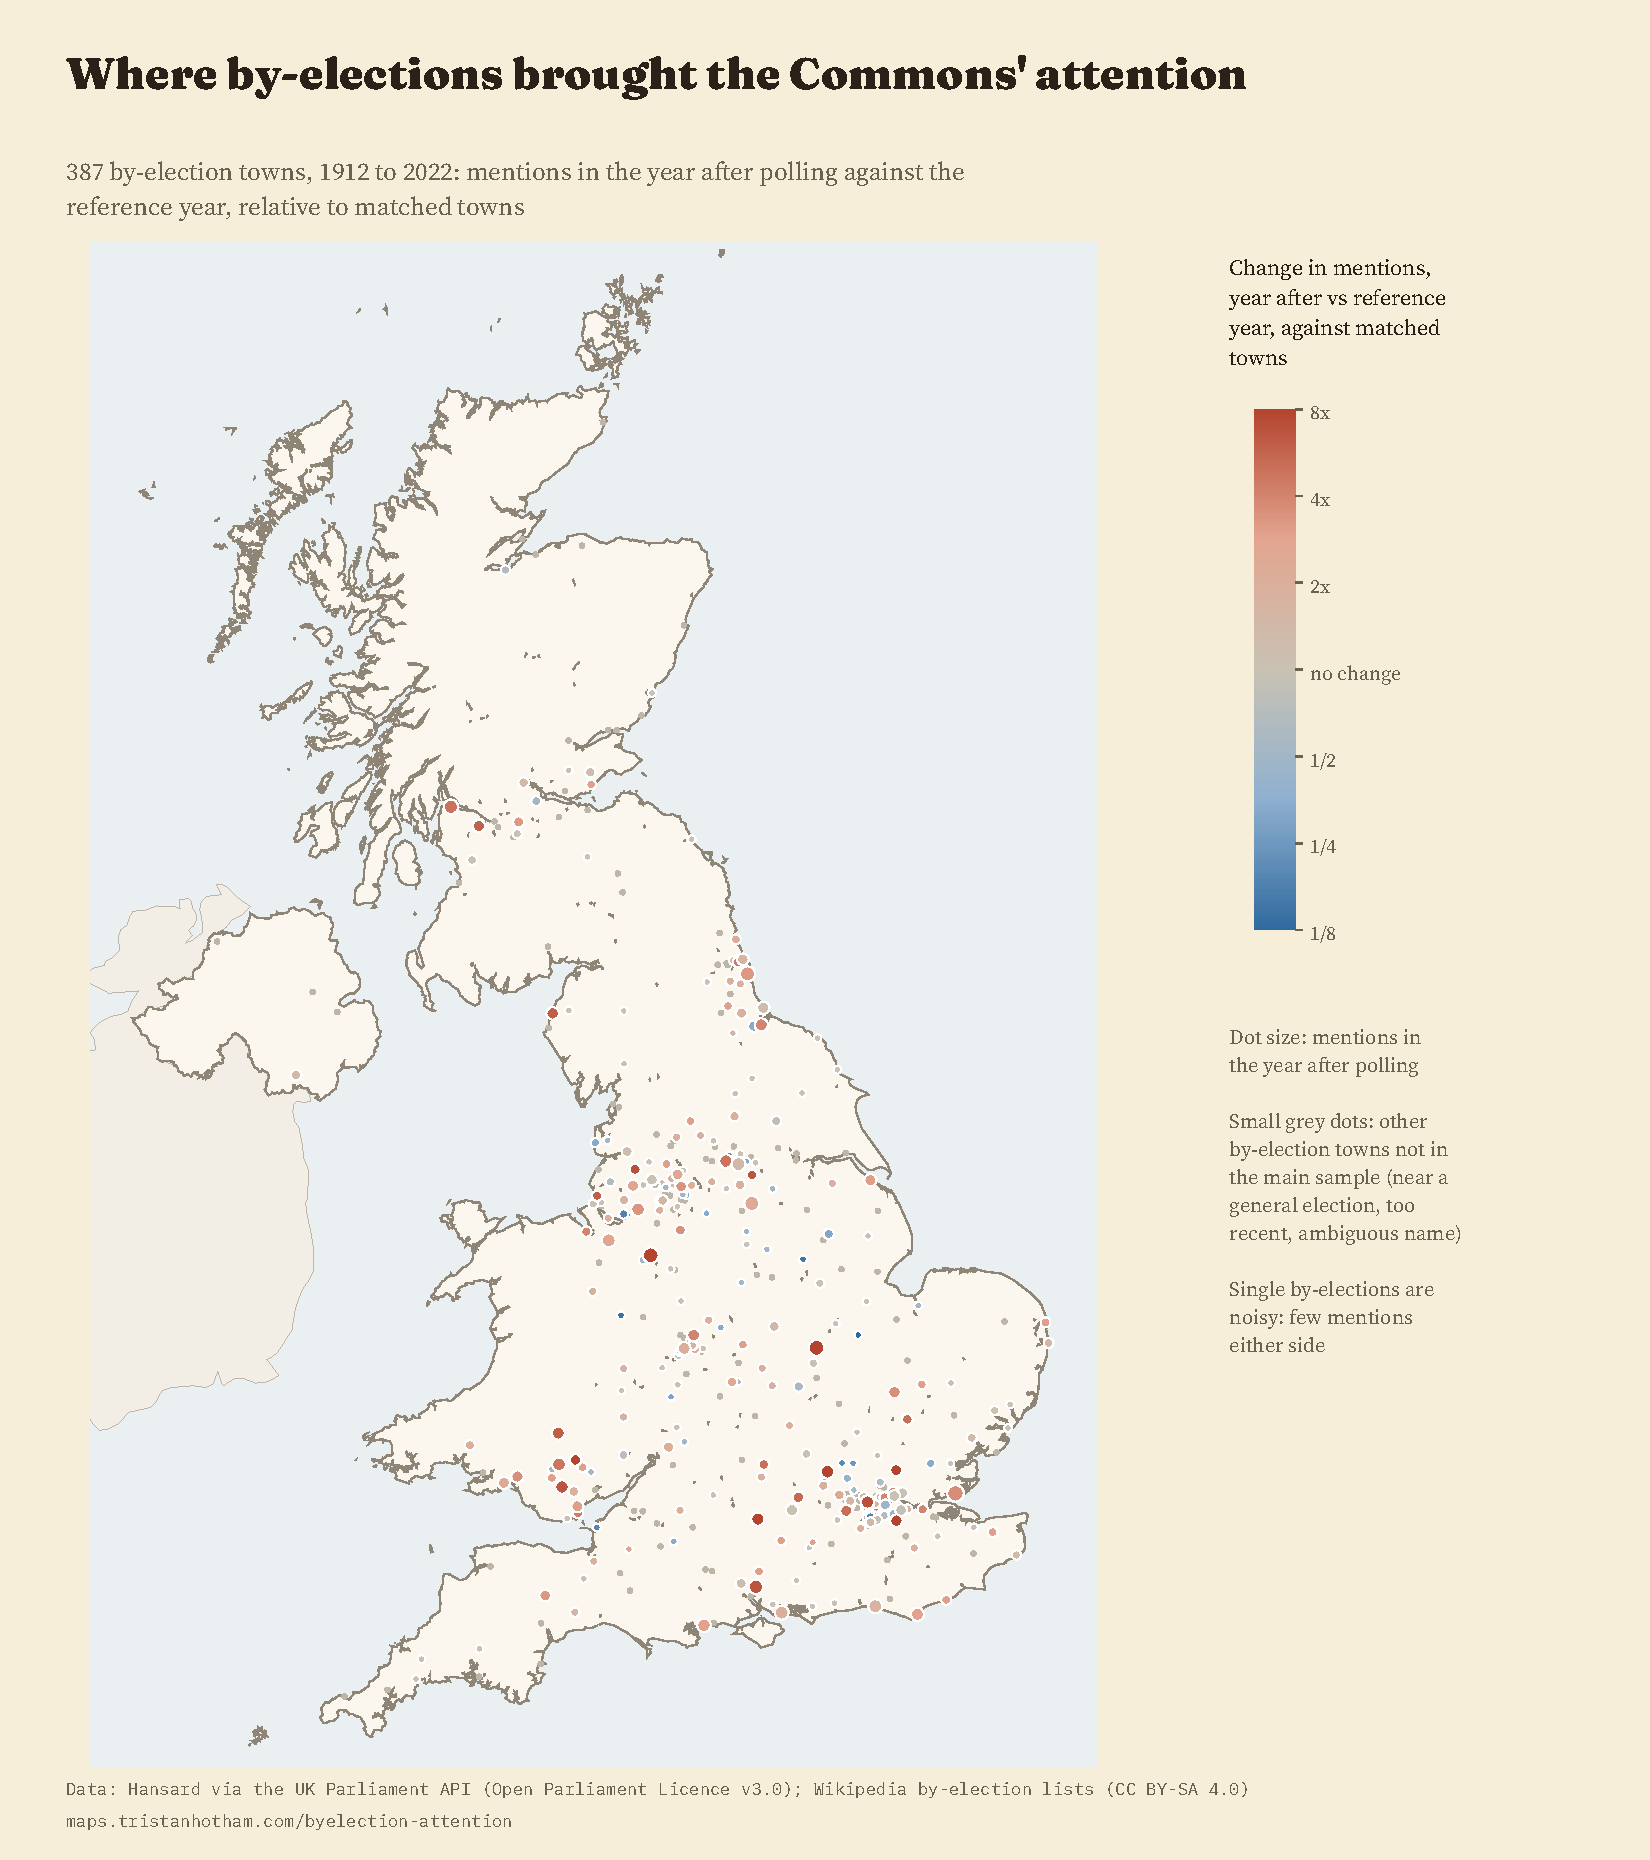
\includegraphics[width=0.86\textwidth]{f_map.pdf}
\caption{Main-sample by-election towns coloured by the ratio of mentions in months 0 to 12 to mentions in months $-24$ to $-13$ (each plus one), divided by the same ratio for the town's five controls; dot size by mentions in months 0 to 12. Grey dots: by-election towns outside the main sample. Single by-elections are noisy; the estimates in the text pool them.}\label{fig:map}
\end{figure}

\subsection{Heterogeneity}
Table~\ref{tab:het} and Figure~\ref{fig:het} report the pre-specified heterogeneity analyses. \textbf{Changing hands (H3).} When the seat changed party (77 towns, 20\% of the sample), mentions in the polling period were 7.1 times those of matched towns, against 3.0 times where the seat was held; the ratio of the two is 2.3 (CI for the difference 27\% to 335\%). A government loss (62 towns) shows the same pattern, 9.1 times against 3.0. But the extra attention of a change of hands does not last: the contrast is 23\% in months 3 to 12 (CI $-$26 to 104) and 40\% in months 13 to 36 (CI $-$23 to 155).

\textbf{Cause (H4).} After a death (187 towns) the rise is large and lasting: 2.43 times in months 3 to 12 and 1.70 times in months 13 to 36. After a resignation or appointment (190 towns) it is smaller and shorter: 1.49 and 1.08 times. The contrast is $-$39\% in months 3 to 12 (CI $-$62 to $-$1) and $-$37\% later (CI $-$60 to $-$0); at the result it is $-$45\% (CI $-$72 to 10). Scandals and voided elections are too few (10 towns) for precise estimates.

\textbf{Era (H5).} The most striking difference is over time. For the 230 towns with by-elections from 1911 to 1944 there is no detectable rise: 24\% in the polling period (CI $-$34 to 133) and about zero thereafter. From 1945 to 1979 (99 towns) the polling-period rise is 163\% and from 1980 to 2023 (58 towns) 590\%; the contrast between the last and the first era is 455\% (CI 162 to 1072), and it persists in months 13 to 36 (113\%, CI 10 to 310).

\textbf{Who held the seat (H6).} Government-held and opposition-held seats do not differ: the contrast is $-$12\% at the result (CI $-$50 to 57), 7\% in months 3 to 12 and $-$8\% later, all with intervals spanning zero.

\textbf{Exploratory splits.} Labelled exploratory in the plan: marginal seats (previous majority under ten points) show a smaller and shorter rise than safer seats, but the contrasts are imprecise; uncontested by-elections (79 towns, all before 1945) show no rise, consistent with the era result; and towns named in only one seat show a larger immediate rise than towns shared between two seats, as expected if the shared towns dilute the signal.

\begin{table}[tbp]\centering\footnotesize\caption{Heterogeneity: percentage change in mentions against matched towns by group, from the stacked PPML with group-specific bins (95\% CI). Contrasts in Appendix Table~\ref{tab:hetfull}.}\label{tab:het}\begin{tabular}{lrlll}\toprule Group & Towns & Months 0 to 2 & Months 3 to 12 & Months 13 to 36\\\midrule
\multicolumn{5}{l}{\textit{Seat result}}\\
\quad held & 310 & 203 [113, 332] & 80 [33, 143] & 28 [$-$5, 73]\\
\quad changed hands & 77 & 612 [330, 1079] & 121 [47, 234] & 80 [7, 202]\\
\multicolumn{5}{l}{\textit{Government}}\\
\quad otherwise & 325 & 204 [119, 322] & 86 [41, 146] & 32 [1, 73]\\
\quad government lost the seat & 62 & 812 [425, 1482] & 111 [29, 246] & 84 [$-$7, 264]\\
\multicolumn{5}{l}{\textit{Seat held by}}\\
\quad government-held & 273 & 320 [176, 538] & 84 [27, 166] & 47 [2, 113]\\
\quad opposition-held & 114 & 272 [151, 449] & 97 [50, 160] & 36 [$-$3, 91]\\
\multicolumn{5}{l}{\textit{Cause}}\\
\quad death & 187 & 408 [248, 642] & 143 [85, 218] & 70 [40, 107]\\
\quad resignation & 190 & 181 [59, 398] & 49 [0, 122] & 8 [$-$28, 62]\\
\quad scandal & 10 & 286 [176, 440] & 55 [$-$14, 180] & 56 [$-$43, 321]\\
\multicolumn{5}{l}{\textit{Era}}\\
\quad 1911 to 1944 & 230 & 24 [$-$34, 133] & 1 [$-$42, 76] & $-$13 [$-$49, 50]\\
\quad 1945 to 1979 & 99 & 163 [76, 293] & 100 [37, 192] & 24 [$-$11, 74]\\
\quad 1980 to 2023 & 58 & 590 [360, 933] & 137 [73, 224] & 86 [28, 169]\\
\multicolumn{5}{l}{\textit{Nation}}\\
\quad England & 334 & 288 [187, 424] & 97 [55, 151] & 49 [15, 94]\\
\quad Scotland & 24 & 345 [22, 1516] & 19 [$-$59, 247] & $-$43 [$-$77, 42]\\
\quad Wales & 28 & 584 [117, 2050] & 129 [9, 383] & 113 [7, 324]\\
\multicolumn{5}{l}{\textit{Previous majority (exploratory)}}\\
\quad marginal (under 10 points) & 88 & 223 [98, 429] & 44 [$-$15, 143] & 8 [$-$36, 84]\\
\quad safer (10 points or more) & 264 & 347 [209, 547] & 117 [71, 175] & 64 [26, 112]\\
\quad unknown & 35 & 136 [21, 358] & 112 [$-$20, 457] & 4 [$-$48, 108]\\
\multicolumn{5}{l}{\textit{Contest (exploratory)}}\\
\quad contested & 308 & 334 [226, 477] & 105 [64, 157] & 52 [18, 94]\\
\quad uncontested & 79 & $-$80 [$-$97, 31] & $-$24 [$-$75, 133] & $-$27 [$-$74, 102]\\
\multicolumn{5}{l}{\textit{Seats naming the town (exploratory)}}\\
\quad one seat & 344 & 400 [245, 624] & 73 [29, 132] & 40 [$-$1, 99]\\
\quad two seats & 43 & 128 [50, 248] & 133 [64, 231] & 47 [8, 100]\\
\bottomrule\end{tabular}\end{table}

\begin{figure}[tbp]\centering
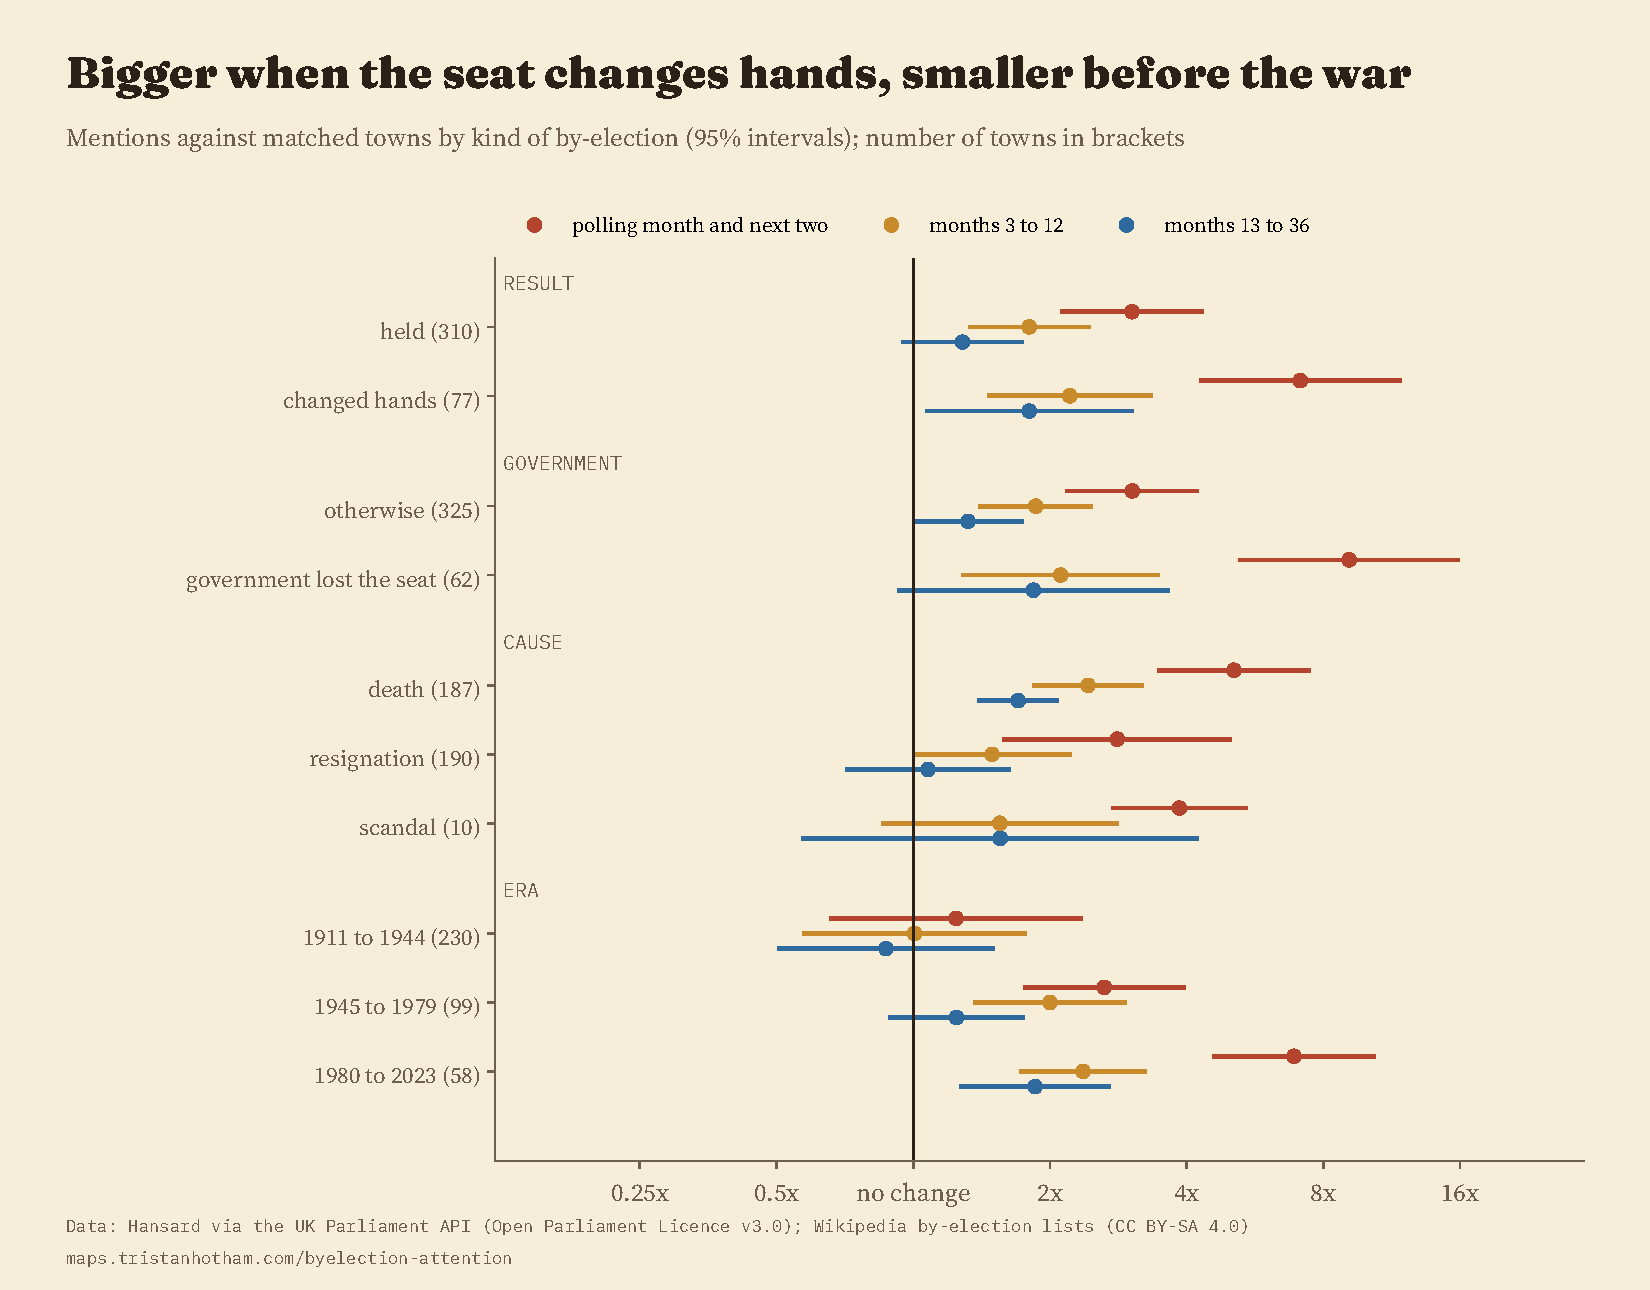
\includegraphics[width=\textwidth]{f_het.pdf}
\caption{Heterogeneity in M1: estimates for the polling period (months 0 to 2), months 3 to 12, and months 13 to 36, by group, with 95\% confidence intervals. Number of by-election towns in brackets.}\label{fig:het}
\end{figure}

\section{Placebos and robustness}\label{sec:robust}
\subsection{Placebos and the seat-name phrase}
Table~\ref{tab:placebo} and Figure~\ref{fig:bins} report the pre-specified placebos. Moving every by-election 24 months earlier and estimating the same model over months $-24$ to $+12$ around the false date (so that the real vacancy falls outside the window) gives estimates close to zero in every bin, for example 8\% at the false polling date (CI $-$18 to 44; 380 towns). Taking up to three towns 3 to 25 km from each by-election town, not named in any seat with a by-election, and treating them as if they had held the by-election, with their own matched controls, gives $-$1\% in the polling period (CI $-$24 to 27; 1,096 towns) and nothing in any other bin: the rise is specific to the place named in the seat, not to its region.

The third placebo, re-elections of the same member, has only 19 by-elections. Mentions in these towns fall rather than rise, already in the pre-period ($-$54\%, CI $-$74 to $-$20), so these few cases are not a clean comparison; they show at least that a by-election with no new member does not bring the rise seen in the main sample.

The seat's own name is a mechanically different measure, because members are named by their seats. It rises only modestly in the polling period (38\%, CI 15 to 65), is lower during the vacancy ($-$18\%, CI $-$33 to 0, when there is no member to name), and is not distinguishable from zero afterwards. This makes it unlikely that the main result reflects the introduction of a new member by the formula ``the hon. Member for''. The comparison also suggests why the formula does not move much: before and after a by-election the seat always has a member to be named, except during the vacancy.

\begin{table}[tbp]\centering\scriptsize\caption{Placebos and the seat-name phrase: percentage change against matched units by period (95\% CI). P1 is estimated over months $-24$ to $+12$ around the false date.}\label{tab:placebo}\setlength{\tabcolsep}{1.5pt}\begin{tabular}{p{2.7cm}rrllllll}\toprule & Units & By-el. & $-12$ to $-4$ & $-3$ to $-1$ & 0 to 2 & 3 to 12 & 13 to 24 & 25 to 36\\\midrule
Main model (M1) & 387 & 366 & 12 [$-$11, 40] & 81 [26, 159] & 296 [196, 429] & 91 [51, 143] & 55 [19, 101] & 31 [$-$1, 73]\\
P1: dates 24 months earlier & 380 & 359 & 16 [$-$8, 46] & $-$16 [$-$38, 15] & 8 [$-$18, 44] & 8 [$-$16, 40] &  & \\
P2: neighbouring towns, 3 to 25 km & 1,096 & 366 & 0 [$-$14, 17] & $-$21 [$-$45, 13] & $-$1 [$-$24, 27] & 5 [$-$19, 37] & $-$15 [$-$35, 11] & $-$13 [$-$30, 8]\\
P3: same member re-elected & 20 & 19 & $-$54 [$-$74, $-$20] & $-$68 [$-$91, 19] & $-$94 [$-$99, $-$64] & $-$85 [$-$92, $-$71] & $-$32 [$-$55, 2] & $-$30 [$-$73, 81]\\
S1: the seat's own name & 366 & 366 & $-$12 [$-$24, 1] & $-$18 [$-$33, 0] & 38 [15, 65] & 13 [$-$6, 36] & 13 [$-$7, 38] & 0 [$-$17, 22]\\
\bottomrule\end{tabular}\end{table}

\begin{figure}[tbp]\centering
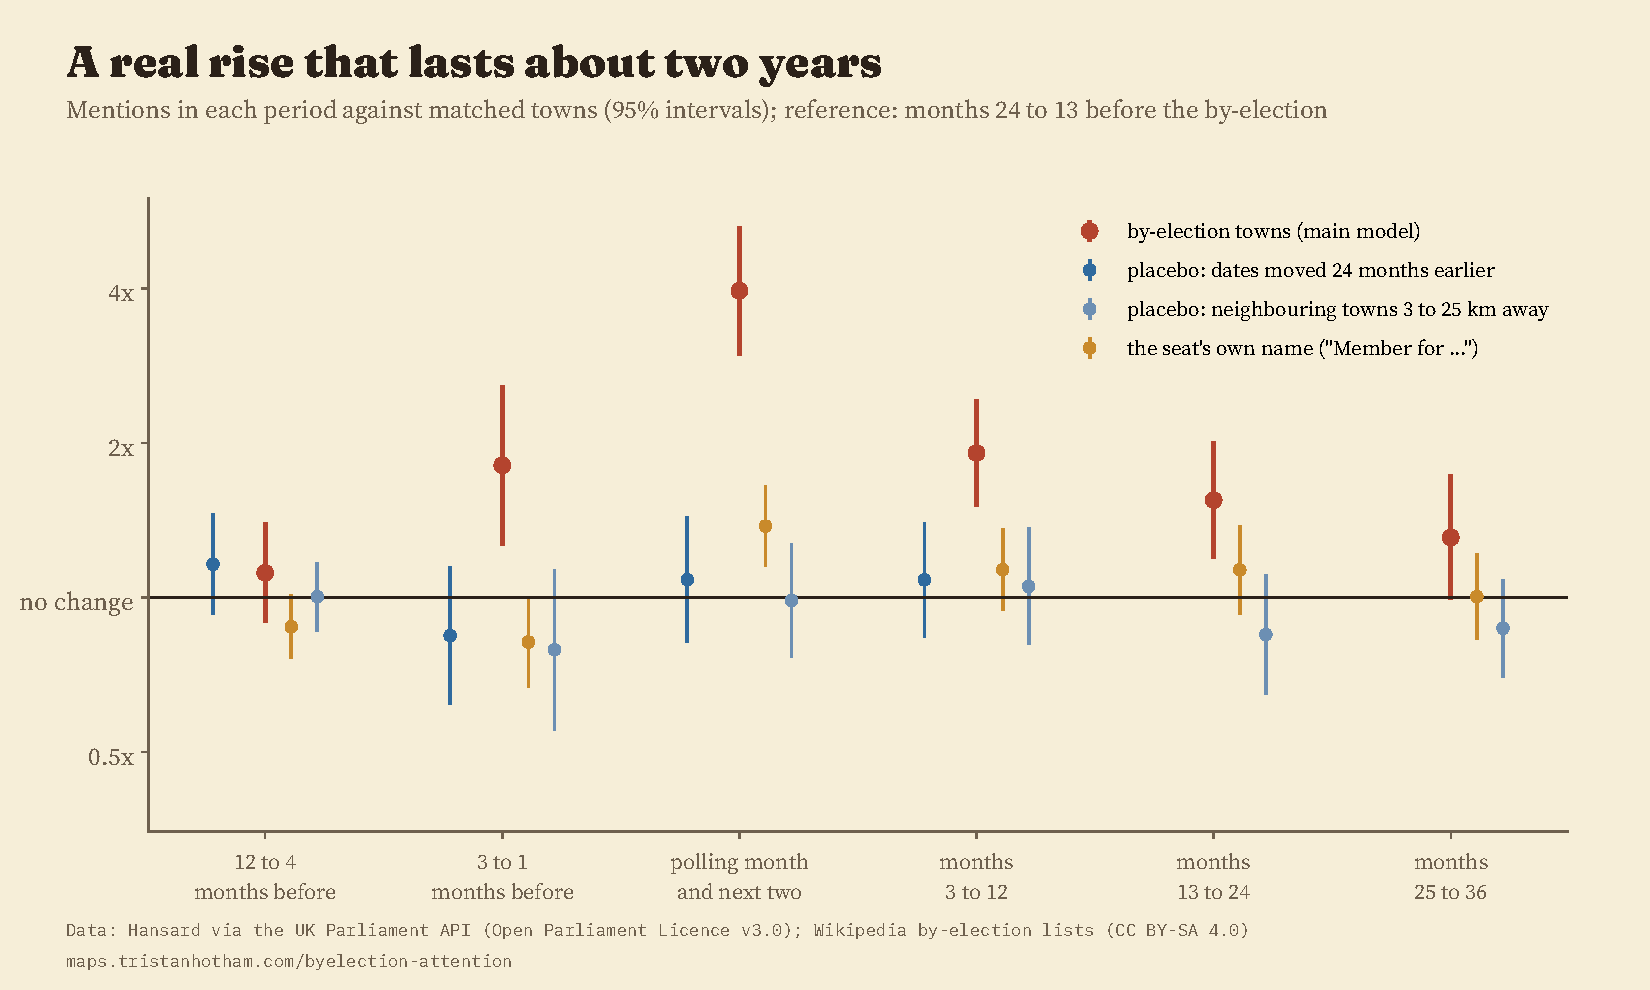
\includegraphics[width=\textwidth]{f_bins.pdf}
\caption{M1 bin estimates (red) against the two placebos (blue) and the seat-name phrase (gold), with 95\% confidence intervals. The fake-date placebo is estimated only up to month 12 after the false date.}\label{fig:bins}
\end{figure}

\subsection{Robustness}
Table~\ref{tab:robust} and Figure~\ref{fig:robust} report every planned check. The polling-period rise is positive with a confidence interval excluding zero in all 18 checks, and the year-1 rise in all but one (leaving out England, which leaves 3,760 usable rows). The year-2 rise is significant in 16 of 18 checks, and the year-3 rise in only 7; I do not treat the third-year estimate as robust. Several checks deserve comment. Clustering by town rather than by-election barely changes the intervals. Ten controls instead of five give very similar estimates. Leaving out each era shows that the later attention depends partly on the post-1980 by-elections: without them, the year-2 estimate is 14\% (CI $-$19 to 60). Including towns divided among three or more seats gives much smaller estimates (polling period 109\%), as expected when the by-election seat is a small part of the place counted. Keeping by-elections near general elections, keeping overlapping by-elections, using only contested by-elections, dropping London, dropping the prefix subtraction and moving the reference period to months $-24$ to $-4$ leave the pattern unchanged. The OLS model of $\log(1+y)$ gives the same pattern on its own (much smaller) scale, as expected for counts dominated by zeros \citep{santos2006}. Two further checks were added at independent review, after the planned analysis, and are exploratory. Because control towns can serve several by-elections, clustering two ways, by by-election and by town, gives almost the same intervals (polling period 296\%, CI 190 to 439; months 25 to 36 31\%, CI $-$2 to 75). Because PPML gives most weight to large counts, dropping the ten by-elections whose towns were mentioned most in months 0 to 12 lowers the later estimates but leaves them positive (polling period 275\%, CI 170 to 419; months 3 to 12 70\%, CI 33 to 117; months 13 to 24 39\%, CI 8 to 79).

\begin{table}[tbp]\centering\scriptsize\caption{Robustness checks: percentage change against matched towns (95\% CI); rows = town-months used. The OLS row reports $100(\exp(b)-1)$ of coefficients on $\log(1+y)$, a different scale.}\label{tab:robust}\setlength{\tabcolsep}{3pt}\begin{tabular}{p{5.6cm}rllll}\toprule Check & Rows & 0 to 2 & 3 to 12 & 13 to 24 & 25 to 36\\\midrule
Main model (M1) & 28,621 & 296 [196, 429] & 91 [51, 143] & 55 [19, 101] & 31 [$-$1, 73]\\
\multicolumn{6}{l}{\textit{Alternative specifications}}\\
\quad OLS of log(1 + mentions) & 141,642 & 15 [12, 19] & 5 [3, 7] & 3 [2, 4] & 2 [1, 4]\\
\quad PPML, treated places only (unit and month fixed effects) & 12,423 & 429 [234, 737] & 142 [47, 300] & 158 [32, 406] & 202 [32, 592]\\
\quad 10 controls per treated place & 63,006 & 301 [206, 426] & 74 [42, 114] & 44 [15, 81] & 27 [$-$1, 62]\\
\multicolumn{6}{l}{\textit{Inference}}\\
\quad Errors clustered by place & 28,621 & 296 [179, 462] & 91 [50, 144] & 55 [16, 106] & 31 [$-$5, 81]\\
\multicolumn{6}{l}{\textit{Leave one out}}\\
\quad Without 1911 to 1944 & 21,831 & 384 [254, 562] & 122 [74, 183] & 76 [33, 134] & 47 [8, 100]\\
\quad Without 1945 to 1979 & 18,171 & 378 [233, 585] & 87 [39, 152] & 64 [19, 128] & 38 [$-$4, 98]\\
\quad Without 1980 to 2023 & 17,240 & 106 [47, 187] & 55 [10, 119] & 14 [$-$19, 60] & 1 [$-$26, 39]\\
\quad Without England & 3,760 & 403 [89, 1240] & 49 [$-$33, 235] & $-$5 [$-$57, 112] & 2 [$-$56, 138]\\
\quad Without Scotland & 26,431 & 298 [197, 432] & 98 [57, 149] & 67 [29, 115] & 39 [5, 84]\\
\quad Without Wales & 27,309 & 288 [188, 422] & 90 [49, 143] & 53 [17, 101] & 29 [$-$4, 72]\\
\quad Without London places & 23,658 & 283 [182, 421] & 98 [53, 154] & 47 [10, 97] & 24 [$-$9, 68]\\
\multicolumn{6}{l}{\textit{Sample and measurement}}\\
\quad Keep by-elections near a general election & 47,347 & 275 [200, 367] & 70 [43, 102] & 45 [21, 73] & 30 [8, 58]\\
\quad Keep overlapping by-elections & 30,519 & 292 [197, 417] & 87 [49, 136] & 51 [17, 95] & 32 [1, 72]\\
\quad Include city divisions (named in 3+ seats) & 42,884 & 109 [71, 156] & 37 [19, 57] & 29 [10, 51] & 17 [$-$0, 36]\\
\quad Contested by-elections only & 26,464 & 334 [226, 477] & 106 [64, 157] & 64 [27, 113] & 40 [6, 85]\\
\quad Places named in one seat only & 21,949 & 408 [250, 637] & 74 [30, 134] & 53 [10, 113] & 29 [$-$13, 91]\\
\quad No prefix subtraction & 28,747 & 293 [194, 425] & 90 [50, 140] & 54 [18, 101] & 30 [$-$1, 72]\\
\quad Reference months $-24$ to $-4$ & 28,621 & 277 [183, 402] & 82 [49, 122] & 47 [19, 82] & 25 [$-$1, 57]\\
\bottomrule\end{tabular}\end{table}

\begin{figure}[tbp]\centering
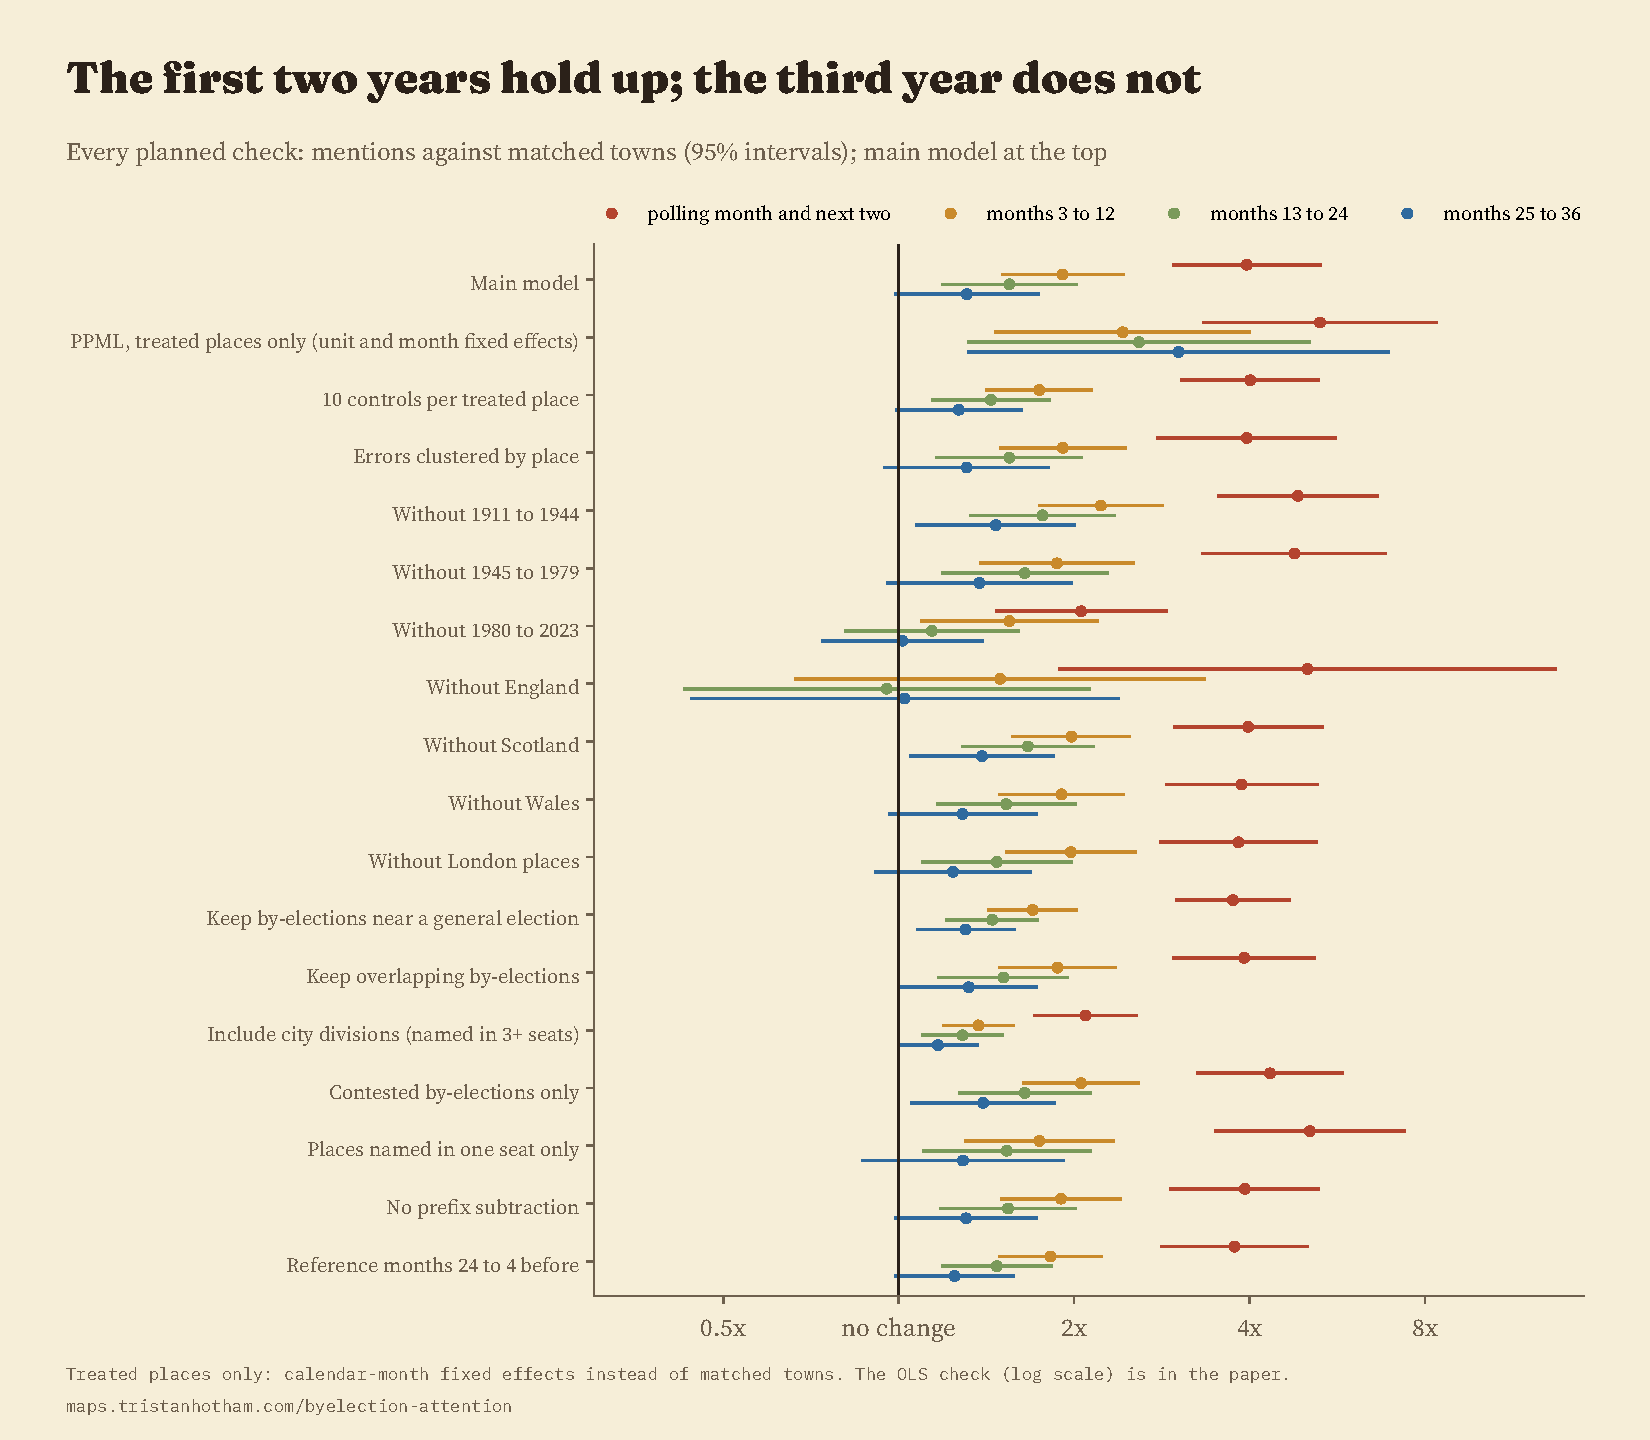
\includegraphics[width=\textwidth]{f_robust.pdf}
\caption{Every planned check: estimates for months 0 to 2, 3 to 12, 13 to 24 and 25 to 36 with 95\% confidence intervals. The OLS check is reported in Table~\ref{tab:robust} only, because its scale differs.}\label{fig:robust}
\end{figure}

\section{Discussion}\label{sec:disc}
\subsection{What the pattern says}
By-elections bring the place to the floor of the House. The rise begins in the vacancy and campaign, reaches its peak at the result, and decays over about two years to a level that, by the third year, is no longer distinguishable from that of similar places. This is not simply the campaign echoing in Westminster: the extra attention in months 3 to 24 is long after the campaign ends, and the placebos show nothing like it in neighbouring towns or at false dates.

What carries the lasting attention? Three mechanisms are consistent with the data, and the counts cannot separate them. The first is the new member: maiden speeches often describe the member's constituency, and a newly elected member has incentives to establish a local profile before the next general election \citep{cain1987,fenno1978}. The larger and longer rise after deaths than after resignations fits this mechanism if members who die in office had, on average, been less active in their final years, so that the new member is a sharper change; but it also fits other explanations, such as the larger shock to local party organisation after a death. The second is the parties: a by-election creates a place that the winners can cite as evidence of support and the losers as a warning, which would explain why the immediate attention is larger when the seat changes hands. That this extra attention fades within months suggests that a by-election upset is a short-lived talking point rather than a lasting change in how the House treats the place. The third is government and the issues the campaign exposed: local problems become national ones for a time. The absence of a difference between government- and opposition-held seats suggests that the attention is not mainly about the government defending its own seats.

The era result is the most substantive. Before 1945 no rise is detectable, even in the polling period. After 1945 the rise is clear, and after 1980 it is larger still. This matches the growth of the constituency role of British MPs described by \citet{norton1994} and \citet{norton1993} and anticipated by \citet{cain1987}: members have come to treat the constituency as a central part of their work and to speak about it in the chamber. It is also consistent with changes in how by-elections are covered, with the arrival of national television coverage of campaigns, and with changes in the House's procedures for questions and adjournment debates. It could reflect changes in the record itself, such as the way older volumes were scanned and indexed. The Hansard series is consistent in its search method, but I cannot rule out that earlier debates use the ``in'' construction differently.

\subsection{Limitations}
First, the design is observational. By-elections are caused by events that may themselves be local news, and the comparison removes stable differences and common shocks but not place-specific events that cause both the vacancy and the attention. The estimates describe the whole episode, not the effect of the vote. Second, the measure is a sample of attention: ``in'' plus the town's name misses mentions by other phrases (``my constituency'', ``the town'') and counts some that refer to the constituency rather than the town; county divisions enter only through the towns in their names, and towns shared among three or more seats are excluded from the main sample. Third, the data do not say who spoke. The leading explanation, a new member speaking for the place, cannot be tested without speaker-level data, which the API's timeline counts do not provide. Fourth, the town list is today's, from a study of present-day places, so the earliest decades and Ireland before 1922 are under-represented, and Northern Ireland contributes a single town to the main sample. Fifth, matching uses a modern population figure for all decades. Sixth, by-election vote shares are not in the lists used here, so swing could not be studied directly; the change of party is used instead. Seventh, scandals and voided elections are few.

\subsection{Implications}
For the study of by-elections, the results suggest that a by-election's consequences go beyond the vote: it raises the place's profile in Parliament for about two years. For the study of representation, they show that constituency attention responds to electoral events in a way that can be measured in debate over a century, and that the strength of that response is itself historical. The design can be extended: to speaker-level counts (to test the new-member mechanism directly), to written questions, to the House of Lords, or to other countries whose parliaments fill vacancies by by-election \citep{loewen2010,studlar1987}.

\section{Conclusion}\label{sec:conc}
Do by-elections make Parliament listen? In one measurable sense, yes. In the House of Commons since 1945, a town whose seat holds a by-election is mentioned several times more often around polling day than similar towns, and about twice as often for the next two years. A change of hands makes the immediate effect larger but not the lasting one, and before 1945 no rise can be detected. The data cannot say how much of this is the new member speaking for home, the parties arguing over the result, or government attending to local problems, but the pattern is clear, specific to the place in the seat's name, and absent where it should be absent. The data and code released with this paper allow the analysis to be rerun and extended.

\section*{Data availability statement}
Data and code: Zenodo DOI https://doi.org/10.5281/zenodo.24094210. The interactive map is at \url{https://maps.tristanhotham.com/byelection-attention/} and the repository at \url{https://github.com/Tristan-Hotham/byelection-attention}. Hansard counts are from the UK Parliament Hansard API (Open Parliament Licence v3.0); the by-election lists from English Wikipedia (CC BY-SA 4.0); the Wikidata check from Wikidata (CC0); town names, points and ambiguity flags from Mentioned in the House \citep{hotham2026a}; seat points and general election dates from Who Won Here? \citep{hotham2026b}.

\section*{AI statement}
I wrote the text, with drafting and editing assistance from Claude (Anthropic), which also helped prepare the analysis code. I reviewed and checked all text and results.

\begin{thebibliography}{99}
\bibitem[Abadie et al.(2023)]{abadie2023} Abadie, A., Athey, S., Imbens, G. W. and Wooldridge, J. M. (2023) When should you adjust standard errors for clustering? \textit{Quarterly Journal of Economics} 138(1), 1 to 35. doi:10.1093/qje/qjac038.
\bibitem[Andr\'e et al.(2015)]{andre2015} Andr\'e, A., Depauw, S. and Martin, S. (2015) Electoral systems and legislators' constituency effort: the mediating effect of electoral vulnerability. \textit{Comparative Political Studies} 48(4), 464 to 496. doi:10.1177/0010414014545512.
\bibitem[Baker et al.(2022)]{baker2022} Baker, A. C., Larcker, D. F. and Wang, C. C. Y. (2022) How much should we trust staggered difference-in-differences estimates? \textit{Journal of Financial Economics} 144(2), 370 to 395. doi:10.1016/j.jfineco.2022.01.004.
\bibitem[Cain et al.(1987)]{cain1987} Cain, B., Ferejohn, J. and Fiorina, M. (1987) \textit{The Personal Vote: Constituency Service and Electoral Independence}. Cambridge, MA: Harvard University Press. doi:10.4159/harvard.9780674493285.
\bibitem[Cameron and Miller(2015)]{cameron2015} Cameron, A. C. and Miller, D. L. (2015) A practitioner's guide to cluster-robust inference. \textit{Journal of Human Resources} 50(2), 317 to 372.
\bibitem[Cengiz et al.(2019)]{cengiz2019} Cengiz, D., Dube, A., Lindner, A. and Zipperer, B. (2019) The effect of minimum wages on low-wage jobs. \textit{Quarterly Journal of Economics} 134(3), 1405 to 1454. doi:10.1093/qje/qjz014.
\bibitem[Cook and Ramsden(1997)]{cook1997} Cook, C. and Ramsden, J. (eds) (1997) \textit{By-Elections in British Politics}, 2nd edn. London: UCL Press. First edition 1973, London: Macmillan.
\bibitem[Correia et al.(2020)]{correia2020} Correia, S., Guimar\~aes, P. and Zylkin, T. (2020) Fast Poisson estimation with high-dimensional fixed effects. \textit{Stata Journal} 20(1), 95 to 115. doi:10.1177/1536867X20909691.
\bibitem[Eulau and Karps(1977)]{eulau1977} Eulau, H. and Karps, P. D. (1977) The puzzle of representation: specifying components of responsiveness. \textit{Legislative Studies Quarterly} 2(3), 233 to 254. doi:10.2307/439340.
\bibitem[Feigert and Norris(1990)]{feigert1990} Feigert, F. B. and Norris, P. (1990) Do by-elections constitute referenda? A four-country comparison. \textit{Legislative Studies Quarterly} 15(2), 183 to 200.
\bibitem[Fenno(1978)]{fenno1978} Fenno, R. F. (1978) \textit{Home Style: House Members in Their Districts}. Boston: Little, Brown.
\bibitem[Fernandes et al.(2018)]{fernandes2018} Fernandes, J. M., Leston-Bandeira, C. and Schwemmer, C. (2018) Election proximity and representation focus in party-constrained environments. \textit{Party Politics} 24(6), 674 to 685. doi:10.1177/1354068817689955.
\bibitem[Hanretty(2021)]{hanretty2021} Hanretty, C. (2021) Forecasting multiparty by-elections using Dirichlet regression. \textit{International Journal of Forecasting} 37(4), 1666 to 1676. doi:10.1016/j.ijforecast.2021.03.007.
\bibitem[Hobolt and Klemmensen(2008)]{hobolt2008} Hobolt, S. B. and Klemmensen, R. (2008) Government responsiveness and political competition in comparative perspective. \textit{Comparative Political Studies} 41(3), 309 to 337. doi:10.1177/0010414006297169.
\bibitem[Hotham(2026a)]{hotham2026a} Hotham, T. (2026a) \textit{Mentioned in the House: which places does Parliament talk about? Place mentions in House of Commons debates, 1909 to 2026}. Zenodo. doi:10.5281/zenodo.23761431.
\bibitem[Hotham(2026b)]{hotham2026b} Hotham, T. (2026b) \textit{Who Won Here? UK general election results by constituency, 1832 to 2024}. Zenodo. doi:10.5281/zenodo.23761425.
\bibitem[Jones and Baumgartner(2005)]{jones2005} Jones, B. D. and Baumgartner, F. R. (2005) \textit{The Politics of Attention: How Government Prioritizes Problems}. Chicago: University of Chicago Press.
\bibitem[Kellermann(2016)]{kellermann2016} Kellermann, M. (2016) Electoral vulnerability, constituency focus, and parliamentary questions in the House of Commons. \textit{British Journal of Politics and International Relations} 18(1), 90 to 106.
\bibitem[Loewen and Bastien(2010)]{loewen2010} Loewen, P. J. and Bastien, F. (2010) (In)significant elections? Federal by-elections in Canada, 1963 to 2008. \textit{Canadian Journal of Political Science} 43(1), 87 to 105.
\bibitem[Mansbridge(2003)]{mansbridge2003} Mansbridge, J. (2003) Rethinking representation. \textit{American Political Science Review} 97(4), 515 to 528.
\bibitem[Martin(2011)]{martin2011} Martin, S. (2011) Using parliamentary questions to measure constituency focus: an application to the Irish case. \textit{Political Studies} 59(2), 472 to 488.
\bibitem[Mughan(1986)]{mughan1986} Mughan, A. (1986) Toward a political explanation of government vote losses in midterm by-elections. \textit{American Political Science Review} 80(3), 761 to 775.
\bibitem[Mughan(1988)]{mughan1988} Mughan, A. (1988) On the by-election vote of governments in Britain. \textit{Legislative Studies Quarterly} 13(1), 29 to 48.
\bibitem[Norris(1990)]{norris1990} Norris, P. (1990) \textit{British By-Elections: The Volatile Electorate}. Oxford: Clarendon Press.
\bibitem[Norton(1994)]{norton1994} Norton, P. (1994) The growth of the constituency role of the MP. \textit{Parliamentary Affairs} 47(4), 705 to 720.
\bibitem[Norton and Wood(1993)]{norton1993} Norton, P. and Wood, D. M. (1993) \textit{Back from Westminster: British Members of Parliament and Their Constituents}. Lexington: University Press of Kentucky.
\bibitem[Pollock(1941)]{pollock1941} Pollock, J. K. (1941) British by-elections between the wars. \textit{American Political Science Review} 35(3), 519 to 528. doi:10.2307/1948768.
\bibitem[Price and Sanders(1998)]{price1998} Price, S. and Sanders, D. (1998) By-elections, changing fortunes, uncertainty and the mid-term blues. \textit{Public Choice} 95(1), 131 to 148. doi:10.1023/A:1004983108916.
\bibitem[Rheault et al.(2016)]{rheault2016} Rheault, L., Beelen, K., Cochrane, C. and Hirst, G. (2016) Measuring emotion in parliamentary debates with automated textual analysis. \textit{PLoS ONE} 11(12), e0168843. doi:10.1371/journal.pone.0168843.
\bibitem[Russo(2011)]{russo2011} Russo, F. (2011) The constituency as a focus of representation: studying the Italian case through the analysis of parliamentary questions. \textit{Journal of Legislative Studies} 17(3), 290 to 301. doi:10.1080/13572334.2011.595122.
\bibitem[Santos Silva and Tenreyro(2006)]{santos2006} Santos Silva, J. M. C. and Tenreyro, S. (2006) The log of gravity. \textit{Review of Economics and Statistics} 88(4), 641 to 658. doi:10.1162/rest.88.4.641.
\bibitem[Searing(1985)]{searing1985} Searing, D. D. (1985) The role of the good constituency member and the practice of representation in Great Britain. \textit{Journal of Politics} 47(2), 348 to 381.
\bibitem[Searing(1994)]{searing1994} Searing, D. D. (1994) \textit{Westminster's World: Understanding Political Roles}. Cambridge, MA: Harvard University Press.
\bibitem[Soroka et al.(2009)]{soroka2009} Soroka, S., Penner, E. and Blidook, K. (2009) Constituency influence in Parliament. \textit{Canadian Journal of Political Science} 42(3), 563 to 591.
\bibitem[Studlar and Sigelman(1987)]{studlar1987} Studlar, D. T. and Sigelman, L. (1987) Special elections: a comparative perspective. \textit{British Journal of Political Science} 17(2), 247 to 256. doi:10.1017/S0007123400004725.
\bibitem[Sun and Abraham(2021)]{sun2021} Sun, L. and Abraham, S. (2021) Estimating dynamic treatment effects in event studies with heterogeneous treatment effects. \textit{Journal of Econometrics} 225(2), 175 to 199. doi:10.1016/j.jeconom.2020.09.006.
\bibitem[Upton(1991)]{upton1991} Upton, G. J. G. (1991) The impact of by-elections on general elections: England, 1950 to 87. \textit{British Journal of Political Science} 21(1), 108 to 119.
\bibitem[Wikipedia contributors(2026)]{wikipedia2026} Wikipedia contributors (2026) List of United Kingdom by-elections (1900 to 1918; 1918 to 1931; 1931 to 1950; 1950 to 1979; 1979 to 2010; 2010 to present). \textit{English Wikipedia}, retrieved 2026. CC BY-SA 4.0.
\bibitem[Zittel et al.(2019)]{zittel2019} Zittel, T., Nyhuis, D. and Baumann, M. (2019) Geographic representation in party-dominated legislatures: a quantitative text analysis of parliamentary questions in the German Bundestag. \textit{Legislative Studies Quarterly} 44(4), 681 to 711. doi:10.1111/lsq.12238.
\end{thebibliography}

\appendix
\section{Appendix: full tables and data construction}
\begin{table}[tbp]\centering\small\caption{Monthly event-study estimates (Figure~\ref{fig:event}B): percentage change against matched towns, 95\% CI; reference months $-24$ to $-13$.}\label{tab:es}\begin{tabular}{rl@{\hskip 24pt}rl}\toprule Month & \% [95\% CI] & Month & \% [95\% CI]\\\midrule
$-$12 & 25 [$-$16, 86] & 13 & 107 [35, 217]\\
$-$11 & 9 [$-$30, 71] & 14 & 121 [44, 237]\\
$-$10 & 23 [$-$27, 108] & 15 & 38 [$-$6, 103]\\
$-$9 & 66 [$-$3, 184] & 16 & 89 [19, 199]\\
$-$8 & $-$12 [$-$39, 29] & 17 & 30 [$-$24, 124]\\
$-$7 & 30 [$-$19, 111] & 18 & 75 [8, 182]\\
$-$6 & 26 [$-$20, 100] & 19 & $-$20 [$-$54, 38]\\
$-$5 & $-$37 [$-$61, $-$0] & 20 & 112 [27, 252]\\
$-$4 & 1 [$-$38, 66] & 21 & 23 [$-$25, 100]\\
$-$3 & $-$10 [$-$47, 52] & 22 & 85 [$-$7, 269]\\
$-$2 & 56 [$-$6, 156] & 23 & 11 [$-$34, 87]\\
$-$1 & 213 [100, 389] & 24 & 48 [$-$6, 134]\\
0 & 487 [308, 744] & 25 & 40 [$-$6, 110]\\
1 & 264 [159, 413] & 26 & 70 [10, 163]\\
2 & 130 [40, 276] & 27 & 108 [5, 313]\\
3 & 149 [63, 282] & 28 & 75 [3, 198]\\
4 & 90 [21, 198] & 29 & 2 [$-$38, 70]\\
5 & 46 [$-$2, 117] & 30 & $-$5 [$-$47, 72]\\
6 & 57 [$-$3, 154] & 31 & 42 [$-$5, 114]\\
7 & 126 [60, 220] & 32 & 31 [$-$4, 79]\\
8 & 119 [51, 218] & 33 & 28 [$-$28, 126]\\
9 & 156 [67, 295] & 34 & $-$21 [$-$54, 34]\\
10 & 78 [5, 202] & 35 & 7 [$-$29, 61]\\
11 & 98 [15, 239] & 36 & 32 [$-$20, 118]\\
12 & 56 [$-$0, 145] & &\\
\bottomrule\end{tabular}\end{table}

\begin{table}[tbp]\centering\scriptsize\caption{Heterogeneity contrasts: the effect in the first-named group relative to the second-named group, as a percentage difference (95\% CI).}\label{tab:hetfull}\begin{tabular}{p{9.5cm}lll}\toprule Contrast & Period & \% [95\% CI] & $p$\\\midrule
Seat result: held vs changed hands & result & $-$57 [$-$77, $-$21] & 0.007\\
Seat result: held vs changed hands & year1 & $-$19 [$-$51, 35] & 0.426\\
Seat result: held vs changed hands & later & $-$29 [$-$61, 30] & 0.267\\
Government: otherwise vs government lost the seat & result & $-$67 [$-$82, $-$37] & 0.001\\
Government: otherwise vs government lost the seat & year1 & $-$12 [$-$50, 55] & 0.661\\
Government: otherwise vs government lost the seat & later & $-$28 [$-$66, 49] & 0.376\\
Seat held by: opposition-held vs government-held & result & $-$12 [$-$50, 57] & 0.676\\
Seat held by: opposition-held vs government-held & year1 & 7 [$-$32, 70] & 0.766\\
Seat held by: opposition-held vs government-held & later & $-$8 [$-$44, 52] & 0.758\\
Cause: resignation vs death & result & $-$45 [$-$72, 10] & 0.090\\
Cause: resignation vs death & year1 & $-$39 [$-$62, $-$1] & 0.046\\
Cause: resignation vs death & later & $-$37 [$-$60, $-$0] & 0.048\\
Cause: scandal vs death & result & $-$24 [$-$54, 26] & 0.284\\
Cause: scandal vs death & year1 & $-$36 [$-$67, 22] & 0.177\\
Cause: scandal vs death & later & $-$9 [$-$67, 152] & 0.861\\
Era: 1945 to 1979 vs 1911 to 1944 & result & 112 [0, 347] & 0.049\\
Era: 1945 to 1979 vs 1911 to 1944 & year1 & 99 [1, 290] & 0.046\\
Era: 1945 to 1979 vs 1911 to 1944 & later & 43 [$-$24, 170] & 0.272\\
Era: 1980 to 2023 vs 1911 to 1944 & result & 455 [162, 1072] & 0.000\\
Era: 1980 to 2023 vs 1911 to 1944 & year1 & 135 [24, 346] & 0.009\\
Era: 1980 to 2023 vs 1911 to 1944 & later & 113 [10, 310] & 0.024\\
Nation: Scotland vs England & result & 15 [$-$70, 331] & 0.840\\
Nation: Scotland vs England & year1 & $-$40 [$-$80, 80] & 0.366\\
Nation: Scotland vs England & later & $-$62 [$-$85, $-$1] & 0.047\\
Nation: Wales vs England & result & 76 [$-$46, 476] & 0.349\\
Nation: Wales vs England & year1 & 16 [$-$47, 154] & 0.710\\
Nation: Wales vs England & later & 43 [$-$32, 198] & 0.342\\
Previous majority (exploratory): safer (10 points or more) vs marginal (under 10 points) & result & 38 [$-$25, 156] & 0.302\\
Previous majority (exploratory): safer (10 points or more) vs marginal (under 10 points) & year1 & 50 [$-$15, 167] & 0.163\\
Previous majority (exploratory): safer (10 points or more) vs marginal (under 10 points) & later & 51 [$-$16, 172] & 0.172\\
Previous majority (exploratory): unknown vs marginal (under 10 points) & result & $-$27 [$-$68, 67] & 0.453\\
Previous majority (exploratory): unknown vs marginal (under 10 points) & year1 & 47 [$-$51, 341] & 0.494\\
Previous majority (exploratory): unknown vs marginal (under 10 points) & later & $-$4 [$-$60, 129] & 0.930\\
Contest (exploratory): uncontested vs contested & result & $-$95 [$-$99, $-$69] & 0.002\\
Contest (exploratory): uncontested vs contested & year1 & $-$63 [$-$88, 16] & 0.088\\
Contest (exploratory): uncontested vs contested & later & $-$52 [$-$83, 37] & 0.170\\
Seats naming the town (exploratory): two seats vs one seat & result & $-$54 [$-$74, $-$19] & 0.007\\
Seats naming the town (exploratory): two seats vs one seat & year1 & 34 [$-$15, 112] & 0.206\\
Seats naming the town (exploratory): two seats vs one seat & later & 5 [$-$34, 67] & 0.848\\
\bottomrule\end{tabular}\end{table}

\textbf{Decisions made by hand.} Seat aliases: ``The Hartlepools'' to Hartlepool; Stratford-on-Avon to Stratford-upon-Avon. Links removed: Colne Valley to Colne; Liverpool West Derby to Derby; Plymouth Sutton to Sutton; Kincardine and Deeside to Deeside. Links kept despite a distant seat point: Merthyr; Kensington (three seats) and Kennington, with London points replacing Hansard's namesake points. Cause groups: every by-election coded as scandal or voided election was read; two appointments (Master in Lunacy; a member certified insane) were moved out of the scandal group. The government in office at each date is coded in \texttt{code/common.py}; Ulster Unionists are treated as Conservatives until March 1972 and Coalition Liberals as part of the government from 1915 to 1922. No by-election or town was dropped by hand for any reason related to the outcome.

\textbf{Software.} Python 3 with pandas, numpy, pyfixest (PPML and OLS with high-dimensional fixed effects), matplotlib and xelatex. All code is in the repository and the data and code archive.

\end{document}
